Actualmente, la predicción climática aún es un reto \cite{Materia_2024}. No obstante, en trabajos previos como los de Elnesr \textit{et al.} \cite{Elnesr_2016, Elnesr_2013} se han desarrollado metodologías deterministas para pronosticar temporadas óptimas para la siembra de distintos tipos de cultivos. Lo anterior, basándose en el concepto de unidades de calor, donde el sistema de unidades de calor se basa en la acumulación promedio de las temperaturas diarias y los umbrales de temperatura respectivos al tipo de cultivo \cite{Chen_1973}.\\

Similarmente, existen más metodologías que basan su análisis únicamente en datos de temperaturas; por ejemplo, los trabajos de Flores--Gallardo \textit{et al.} (2012) \cite{Flores-Gallardo_2012}, Narayan \textit{et al.} (2014) \cite{Narayan_2014} y Callejas--Rodríguez \textit{et al.} (2023) \cite{Callejas-Rodriguez_2023}. Más aún, tales metodologías han sido aplicadas en zonas de cultivo para evaluar su efectividad y comparar los resultados que se obtienen con la implementación de las distintas metodologías.\\



De acuerdo con registros de producción agrícola de 2023 del Servicio de Información Agroalimentaria y Pesquera (SIAP), disponibles en \url{http://infosiap.siap.gob.mx/gobmx/datosAbiertos.php}, el estado de Michoacán es considerado como el principal productor de aguacate a nivel nacional, siendo Tancátaro, Tacámbaro, Uruapan, Ario y Peribán los municipios con mayor valor de producción. Por tanto, al focalizar el análisis en esta zona geográfica, podríamos garantizar los niveles de producción a largo plazo.\\

Más aún, al incorporar de manera conjunta tanto datos edáficos, eólicos e hídricos, así como también las unidades de calor, podríamos esperar resultados más detallados al considerar las metodologías de aprendizaje automático. En específico, la plataforma Essenger \cite{Rodriguez-Moreno_2021}, del Instituto Nacional de Investigaciones Forestales, Agrícolas y Pecuarias (INIFAP), alberga datos históricos diarios, desde 1980 a 2022, de temperatura máxima y mínima del aire, horas de luz, radiación de onda corta, lluvia líquida y presión del vapor de agua.\\

Asimismo, la plataforma Malla Suelos México, del INIFAP y disponible en \url{https://clima.inifap.gob.mx/lnmysr/DatosIndirectos/MSMx}, contiene datos del suelo sobre la densidad aparente, contenido de arcilla, capacidad de intercambio catiónico, fragmentos de roca, nitrógeno, densidad de carbono orgánico, arena y sedimento, además del pH del agua. Los datos antes mencionados fueron medidos a distintas profundidades, en un rango de 0 a 200 cm.\\

Adicionalmente, la Comisión Nacional del Agua (CONAGUA), a través del Sistema Meteorológico Nacional (SMN), mantiene registros históricos diarios referentes a la precipitación, evaporación, temperatura máxima y temperatura mínima; tales datos provienen de las estaciones climáticas dispersas por el territorio nacional y son accesibles a través de \url{https://smn.conagua.gob.mx/es/climatologia/informacion-climatologica/normales-climatologicas-por-estado}. Aunado a lo anterior, se tienen datos mensuales de precipitación, temperatura mínima, media y máxima a nivel estatal, los cuales se encuentran disponibles en \url{https://smn.conagua.gob.mx/es/climatologia/temperaturas-y-lluvias/resumenes-mensuales-de-temperaturas-y-lluvias}.\\ 

De acuerdo con el SIAP \cite{AvanceSiembrasCosechas}, aproximadamente el 60.18 \% de los municipios del estado de Michoacán son productores de aguacates; esto es, un total de 68 municipios destinan zonas de cultivo para la siembra y cosecha de aguacate, ver Figura \ref{fig:Reporte2024}. Como puede apreciarse en la Figura \ref{fig:ProduccionAnual2024}, la participación de los municipios en la producción es desigual, lo cual puede atribuirse a diversos aspectos como la superficie destinada a los cultivos, disponibilidad de recursos, condiciones climáticas, entre otros factores.\\

Por otra parte, se sabe que en promedio un árbol alcanza una producción de hasta 200 kg y que una hectárea tiene la capacidad de albergar 280 árboles \cite{Pena-Urquiza_2015}. De esta manera, al estudiar el rendimiento de las zonas de cultivo, normalizando las toneladas de aguacates producidos respecto a las hectáreas cosechadas, se tiene otra alternativa para medir el impacto que tiene cada municipio dentro de los procesos productivos. Lo anterior se muestra en la Figura \ref{fig:RendimientoAnual2024} y con esto podría ser posible caracterizar las variables agroclimáticas que, potencialmente, favorecen un mayor rendimiento por hectárea.\\

\begin{figure}[ht]
\centering
\subfloat[Producción anual 2024 por municipio.]{\label{fig:ProduccionAnual2024}
\centering
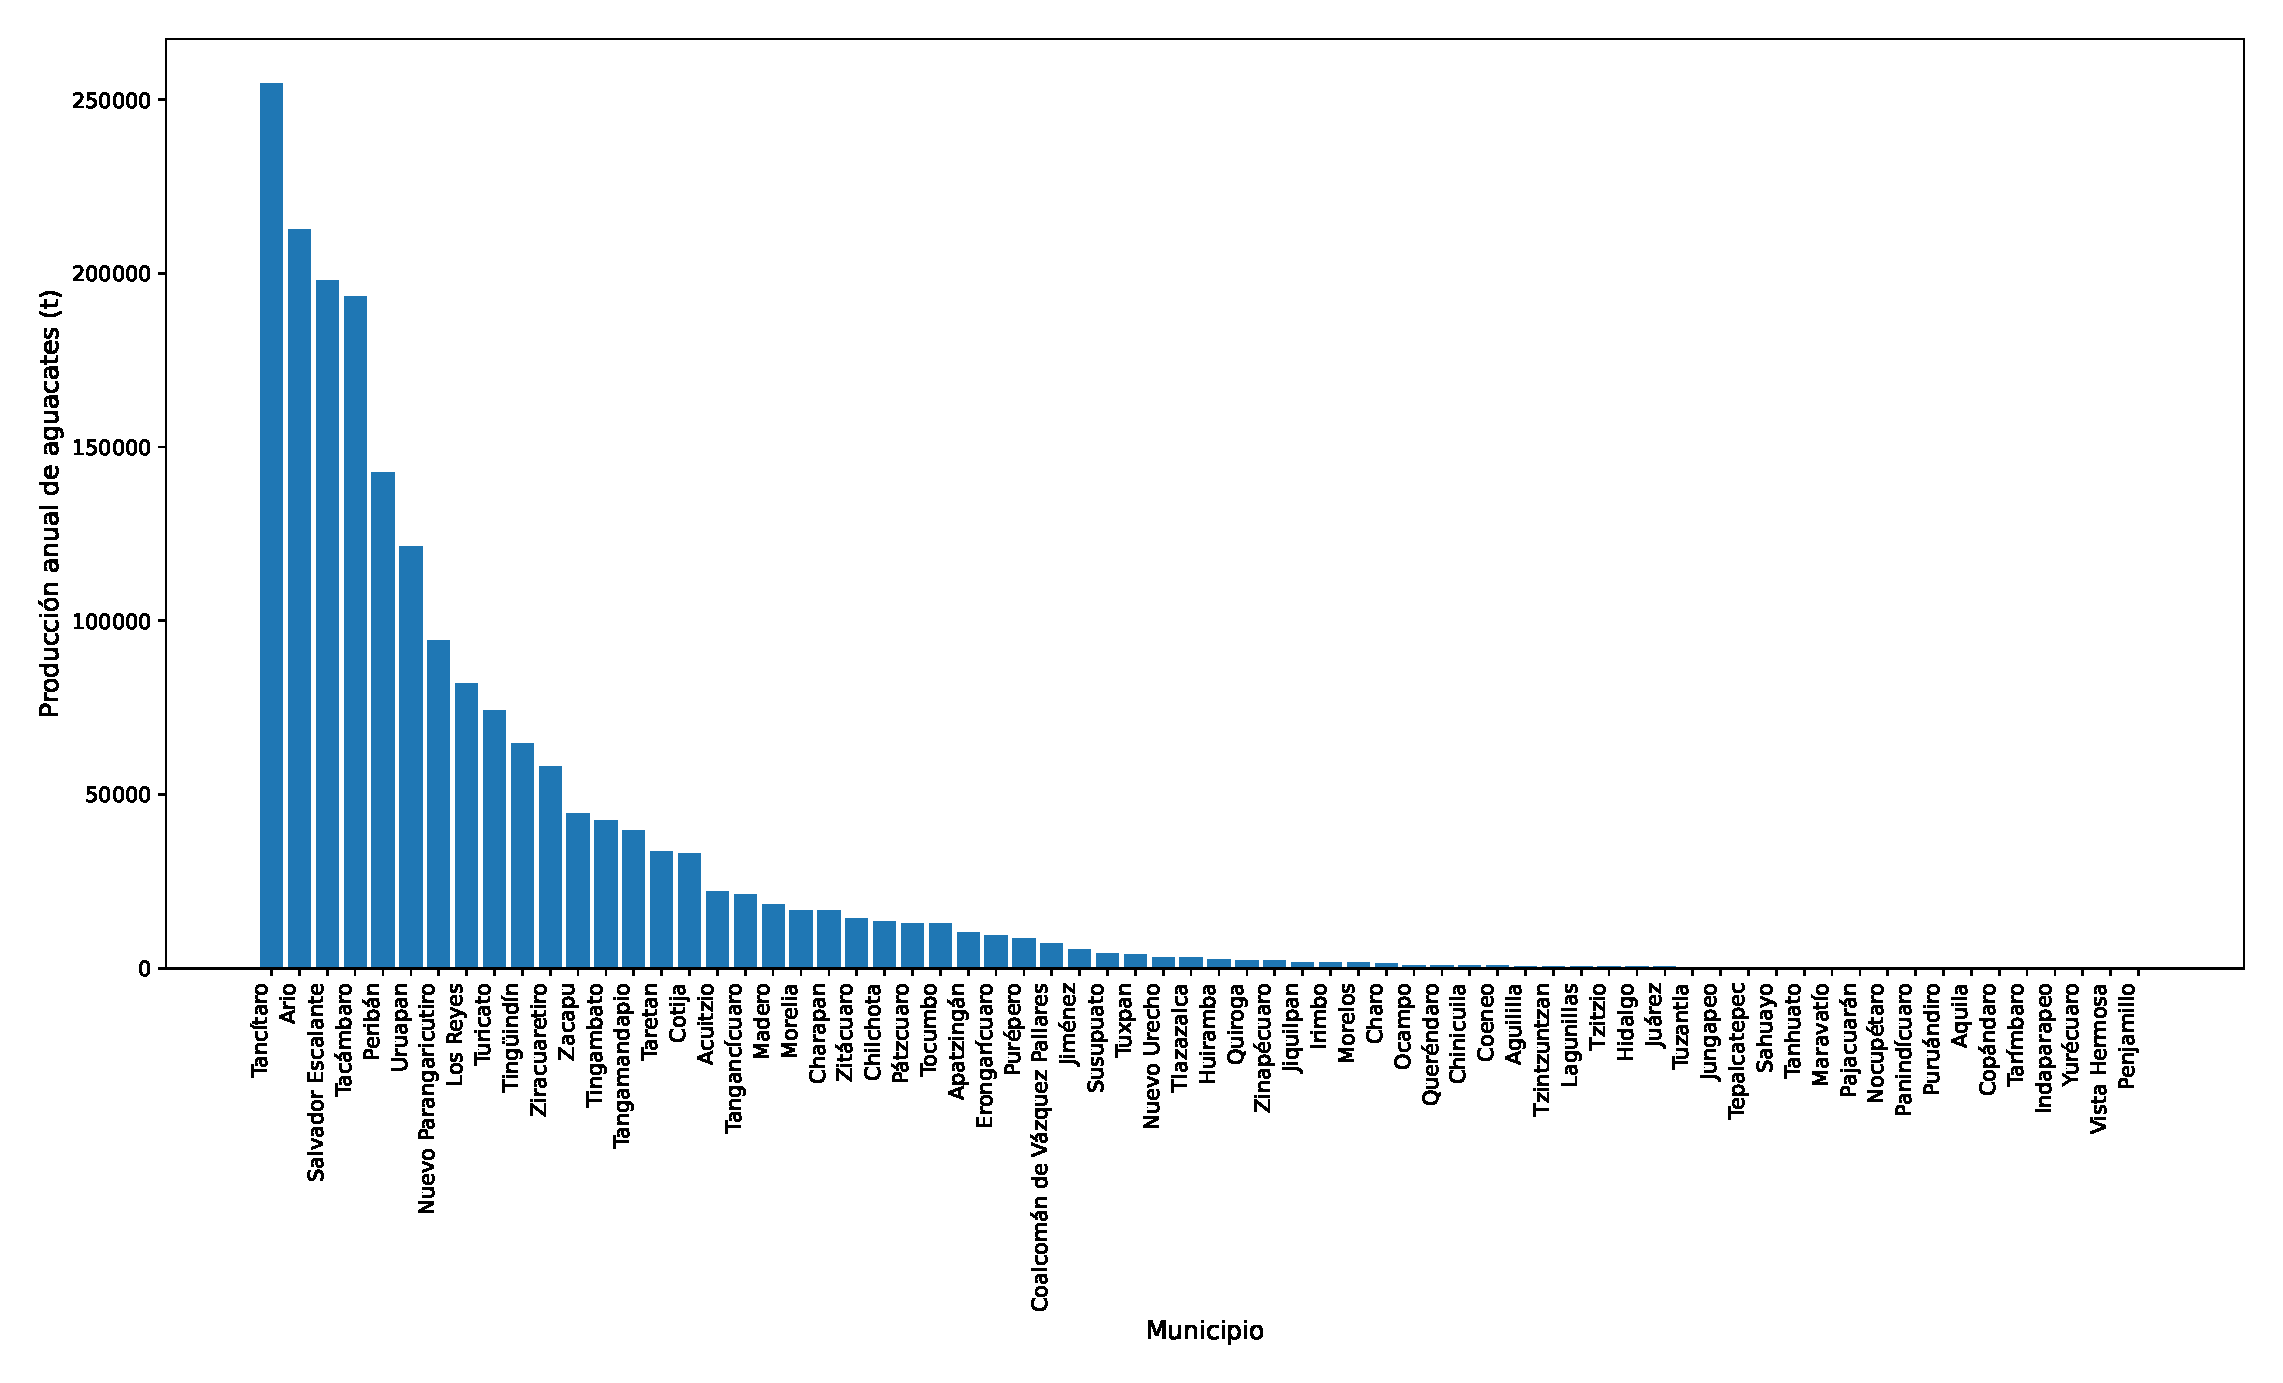
\includegraphics[width=\linewidth]{Images/ProduccionAnual2024.eps}
}
%no space
\hfill
\subfloat[Rendimiento anual 2024 por municipio.]{\label{fig:RendimientoAnual2024}
\centering
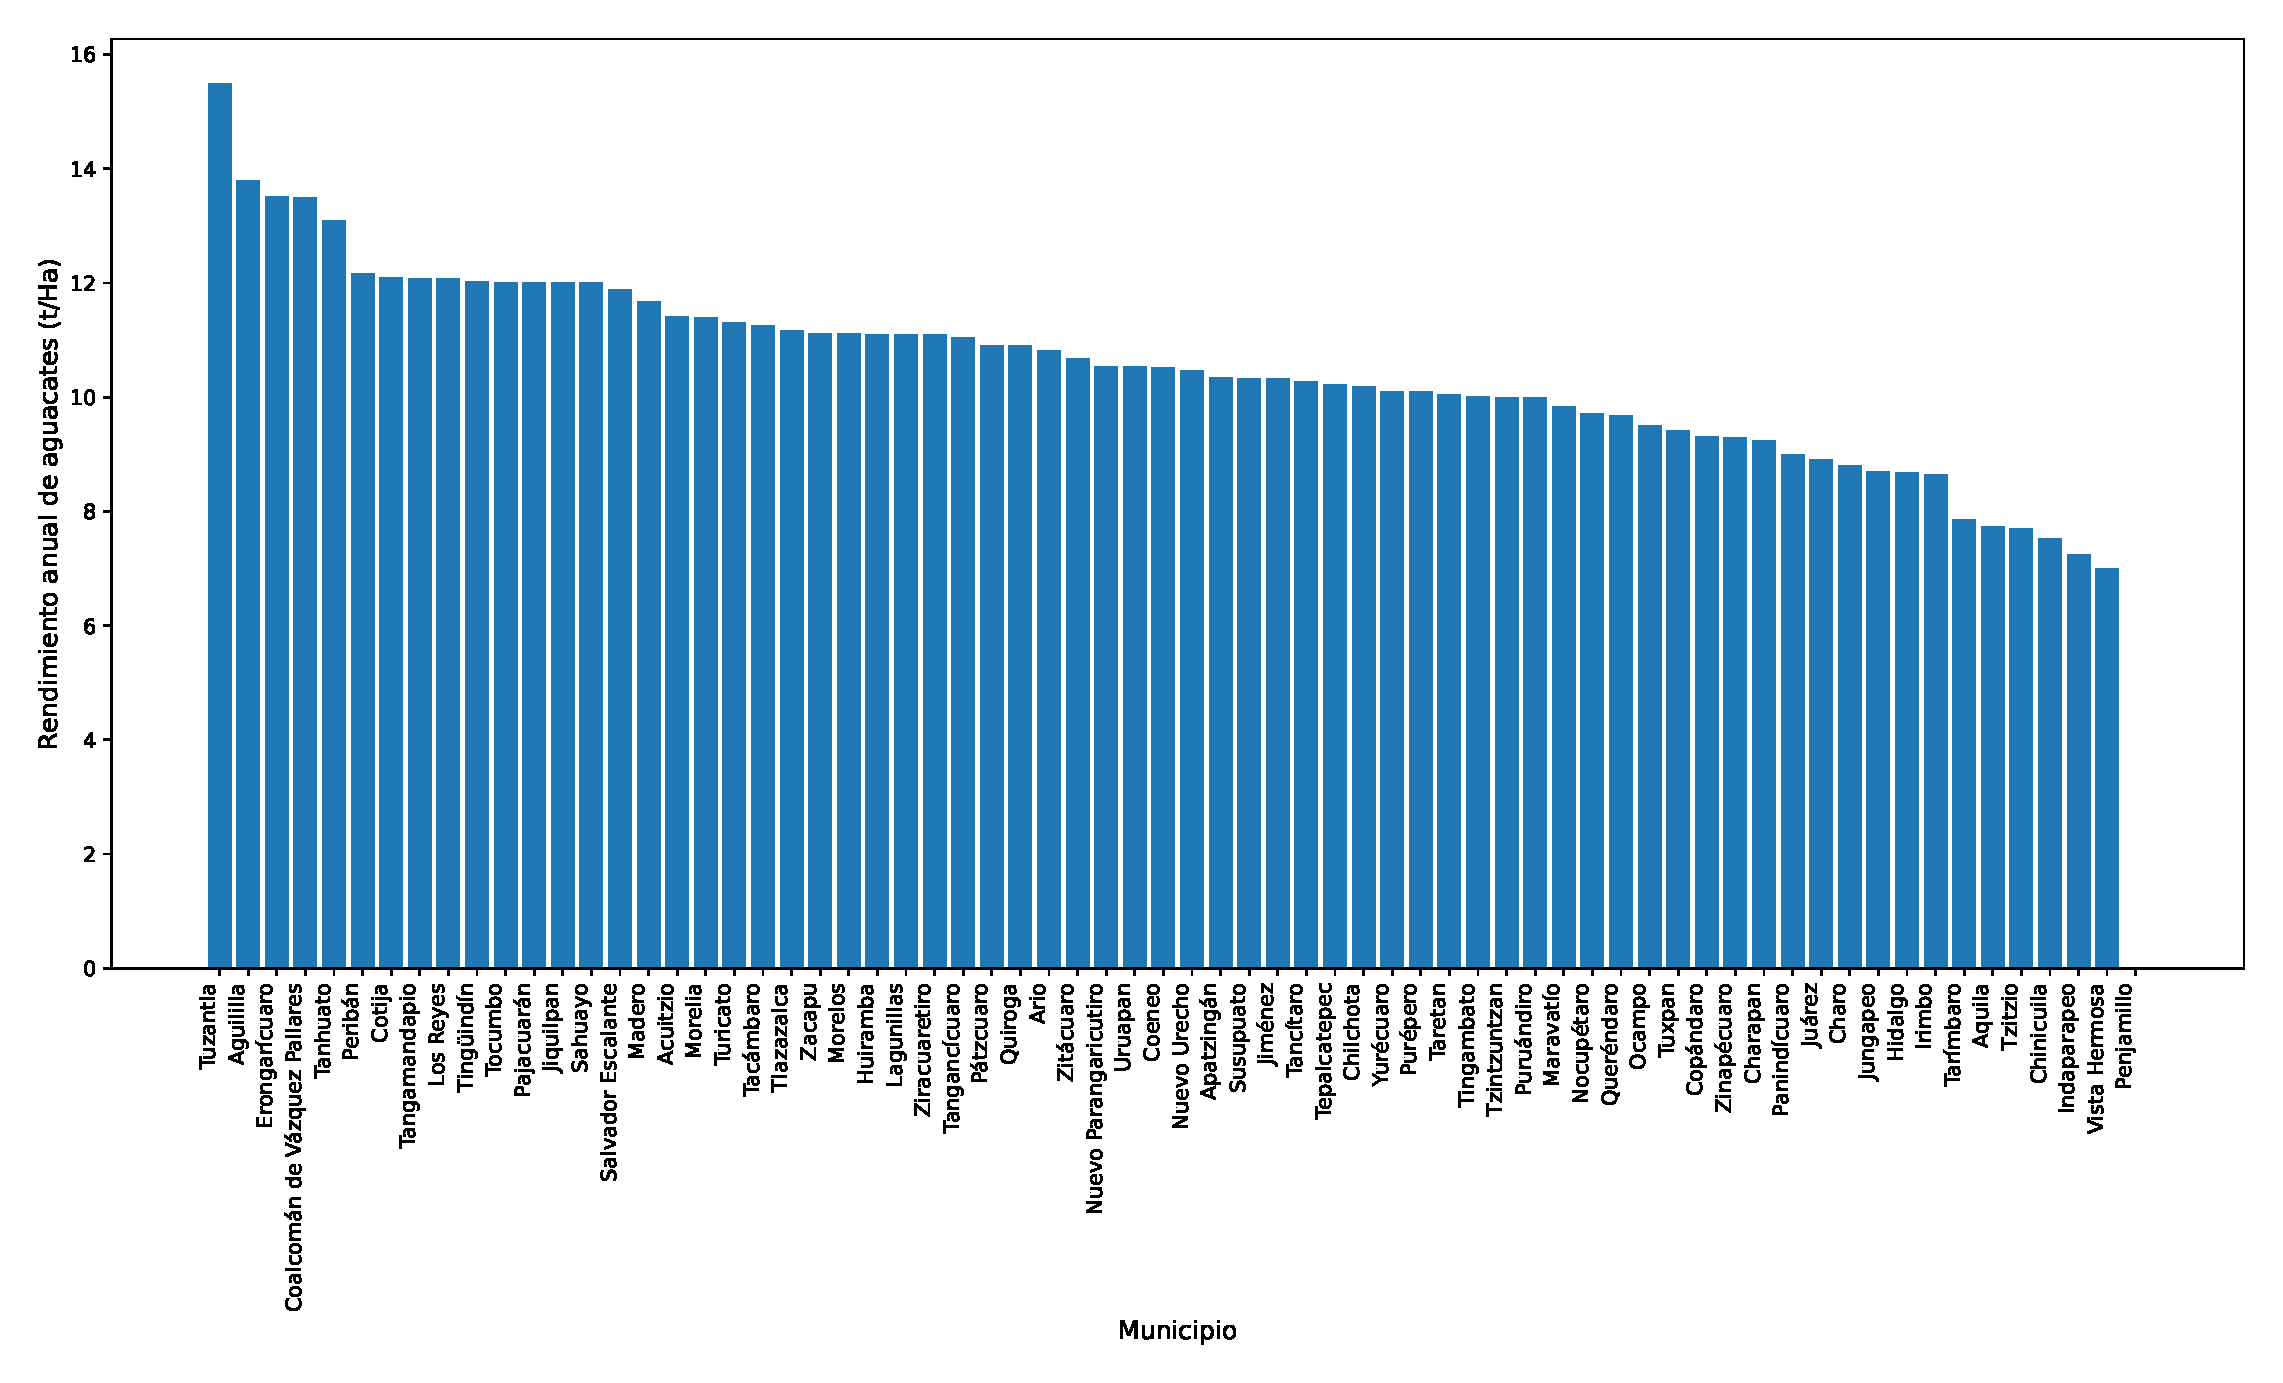
\includegraphics[width=\linewidth]{Images/RendimientoAnual2024.eps}
}
\caption{Reporte de producción y rendimiento anual de aguacates por municipio del 1 de enero al 31 de diciembre de 2024. Figura construida a partir de los datos disponibles en \cite{AvanceSiembrasCosechas}.}
\label{fig:Reporte2024}
\end{figure}



En la Figura \ref{fig:Meteorological_comparison}, presentamos los registros meteorológicos históricos, desde 2012 hasta 2022, obtenidos de \cite{Rodriguez-Moreno_2021} para las estaciones Pedernales y El Varal, ubicadas en el municipio de Tacámbaro y Los Reyes, Michoacán, respectivamente. Por un lado, de acuerdo con la Figura \ref{fig:ProduccionAnual2024}, Tacámbaro ocupa el cuarto lugar a  nivel de producción; mientras que Los Reyes ocupa el octavo lugar. No obstante, al considerar el rendimiento por hectárea que se muestra en la Figura \ref{fig:RendimientoAnual2024}, paradójicamente, se observa que Los Reyes y Tacámbaro se posicionan en el noveno y en el vigésimo primer lugar, respectivamente.\\


Para ilustrar lo anterior, en la Figura \ref{fig:Produccion_comparison_TimeSeries} se muestran los registros históricos desde el 1 de enero de 2018 al 31 de enero de 2025 para cultivos de riego y temporal que pertenecen a los municipios de Tacámbaro y Los Reyes, respectivamente.\\

\begin{figure}[!ht]
    \centering
    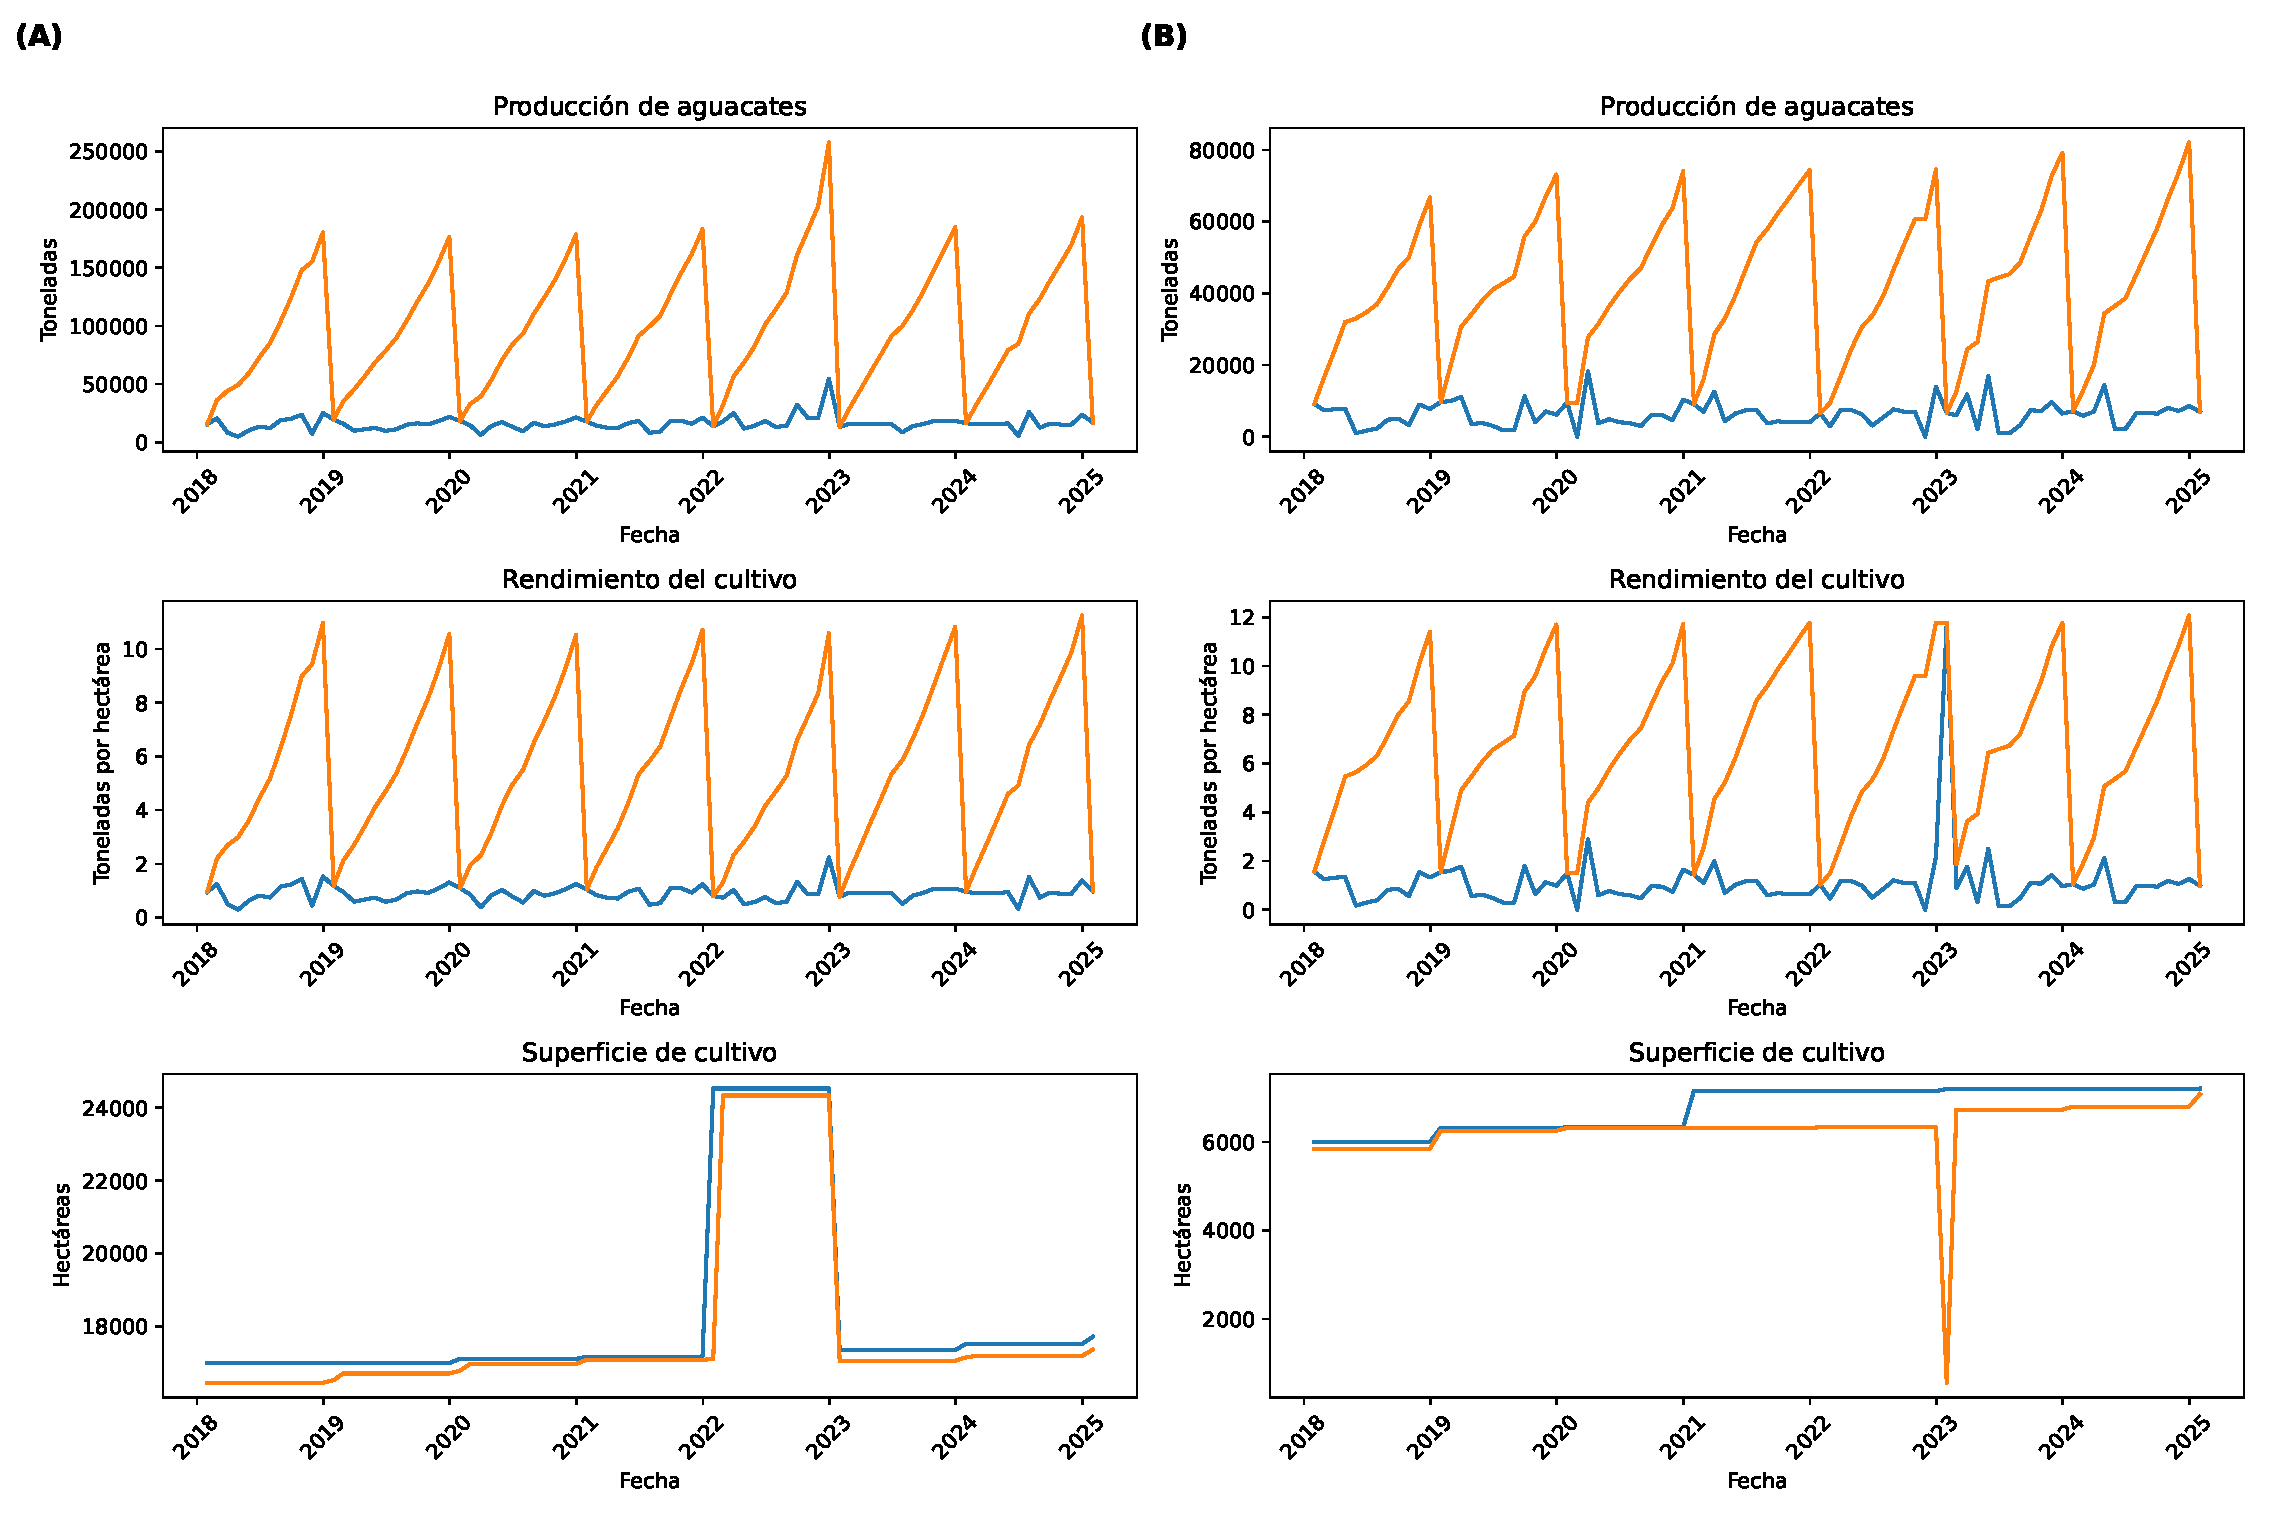
\includegraphics[width=1\linewidth]{Images/Tacámbaro_LosReyes_Comparison.eps}
    \caption{Comparación de producción y rendimiento mensual histórico desde enero de 2018 a enero de 2025 para los municipios de Tacámbaro y Los Reyes. La Figura (\textbf{A}) muestra los datos registrados para Tacámbaro; mientras que, la Figura (\textbf{B}) muestra los datos registrados para Los Reyes. Respecto a la producción de aguacates, en azul se muestra la producción mensual; mientras que, en naranja se ilustra la producción acumulada. Similarmente, respecto al rendimiento del cultivo, en azul se muestra el rendimiento mensual y en naranja el rendimiento acumulado. Por último, respecto a la superficie de cultivo, en azul se muestra el número de hectáreas sembradas; mientras que, en naranja se muestra el número de hectáreas cosechadas. Figura construida a partir de los datos disponibles en \cite{AvanceSiembrasCosechas}.}
    \label{fig:Produccion_comparison_TimeSeries}
\end{figure}

Al considerar los datos anteriores, provenientes de \cite{AvanceSiembrasCosechas}, y en ausencia de la hipótesis de normalidad, la cual se verificó a través de una prueba Shapiro--Wilk ($p <0.05$), la afirmación anterior sobre las diferencias de producción y rendimiento entre ambos municipios puede sustentarse estadísticamente a través de la implementación de pruebas U de Mann--Whitney.\\

\begin{figure}[!ht]
    \centering
    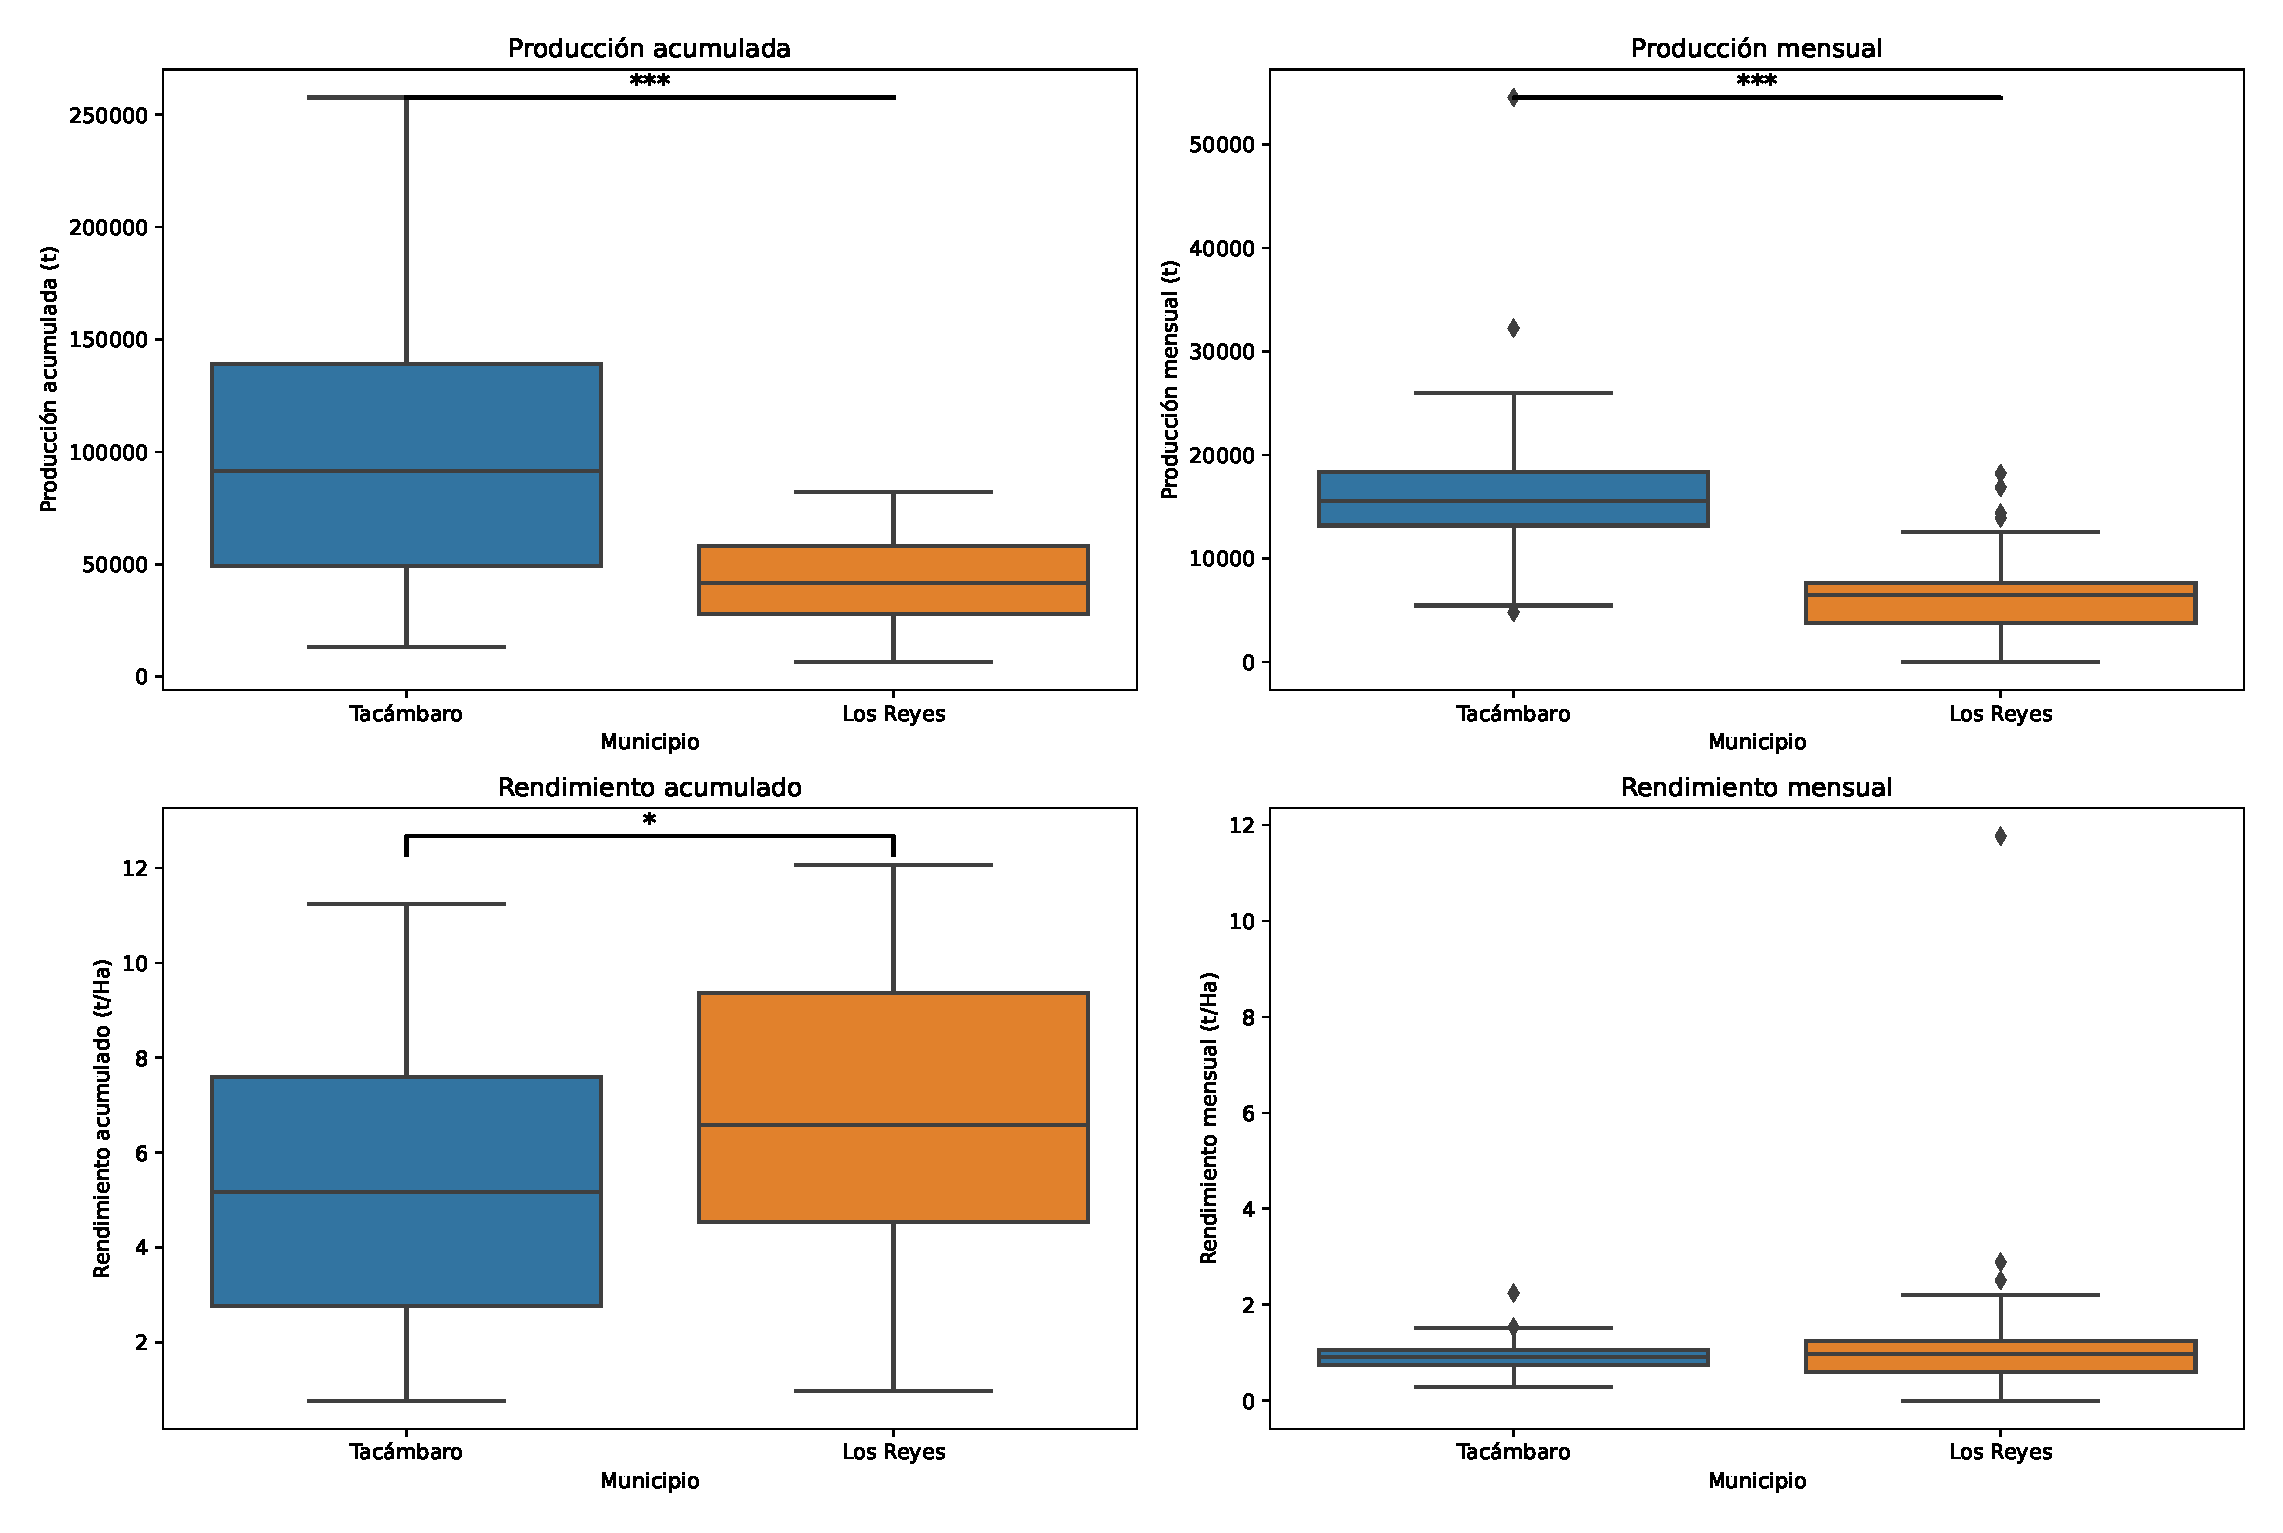
\includegraphics[width=1\linewidth]{Images/Produccion_statistical_comparison.eps}
    \caption{Comparación de producción acumulada, producción mensual, rendimiento acumulado y rendimiento mensual histórico desde enero de 2018 a enero de 2025 para los municipios de Tacámbaro (en azul) y Los Reyes (en naranja). Figura construida a partir de los datos disponibles en \cite{AvanceSiembrasCosechas}.}
    \label{fig:Produccion_comparison}
\end{figure}

Como puede apreciarse en la Figura \ref{fig:Produccion_comparison}, a nivel de producción, en efecto hay diferencias estadísticamente significativas ($p<0.001$) y el resultado es consistente con el análisis mencionado para la Figura \ref{fig:ProduccionAnual2024}. Más aún, en la Figura \ref{fig:Produccion_comparison} se observa que hay diferencias estadísticamente significativas respecto al rendimiento acumulado ($p<0.05$), es decir, aquel que incorpora la producción acumulada mes tras mes y la pondera respecto a la superficie cosechada. Lo anterior es congruente con el análisis mencionado para la Figura \ref{fig:RendimientoAnual2024}.\\

Por otra parte, para el rendimiento mensual, es decir, aquel que considera únicamente las toneladas producidas a lo largo de cada mes y las pondera respecto a la superficie cosechada de dicho mes, no hay evidencia de diferencias estadísticamente significativas. Esto podría indicar que a escalas de tiempo cortas, el rendimiento no es una medida tan relevante o informativa, pero a escalas de tiempo largas puede darnos indicios sobre las características que intervienen en los niveles de producción por hectárea.\\



Notemos que, derivado de su cercanía geográfica, los municipios productores del estado de Michoacán cuentan con similitudes en tanto a los recursos, las características agrometeorológicas y más propiedades biológicas. No obstante, fenómenos como la orografía o la actividad humana intervienen en enfatizar o diluir tales similitudes.\\

Por tanto, a manera de análisis exploratorio, estudiaremos el efecto de la duración en segundos del periodo luminoso diario, las precipitaciones diarias, la radiación solar de onda corta diaria, la temperatura máxima del aire, la temperatura mínima del aire y la presión del vapor de agua diaria sobre los niveles de producción y rendimiento del aguacate, tanto para el municipio de Tacámbaro como para el municipio de Los Reyes, ver Figura \ref{fig:Meteorological_comparison}.\\


\begin{figure}[!ht]
    \centering
    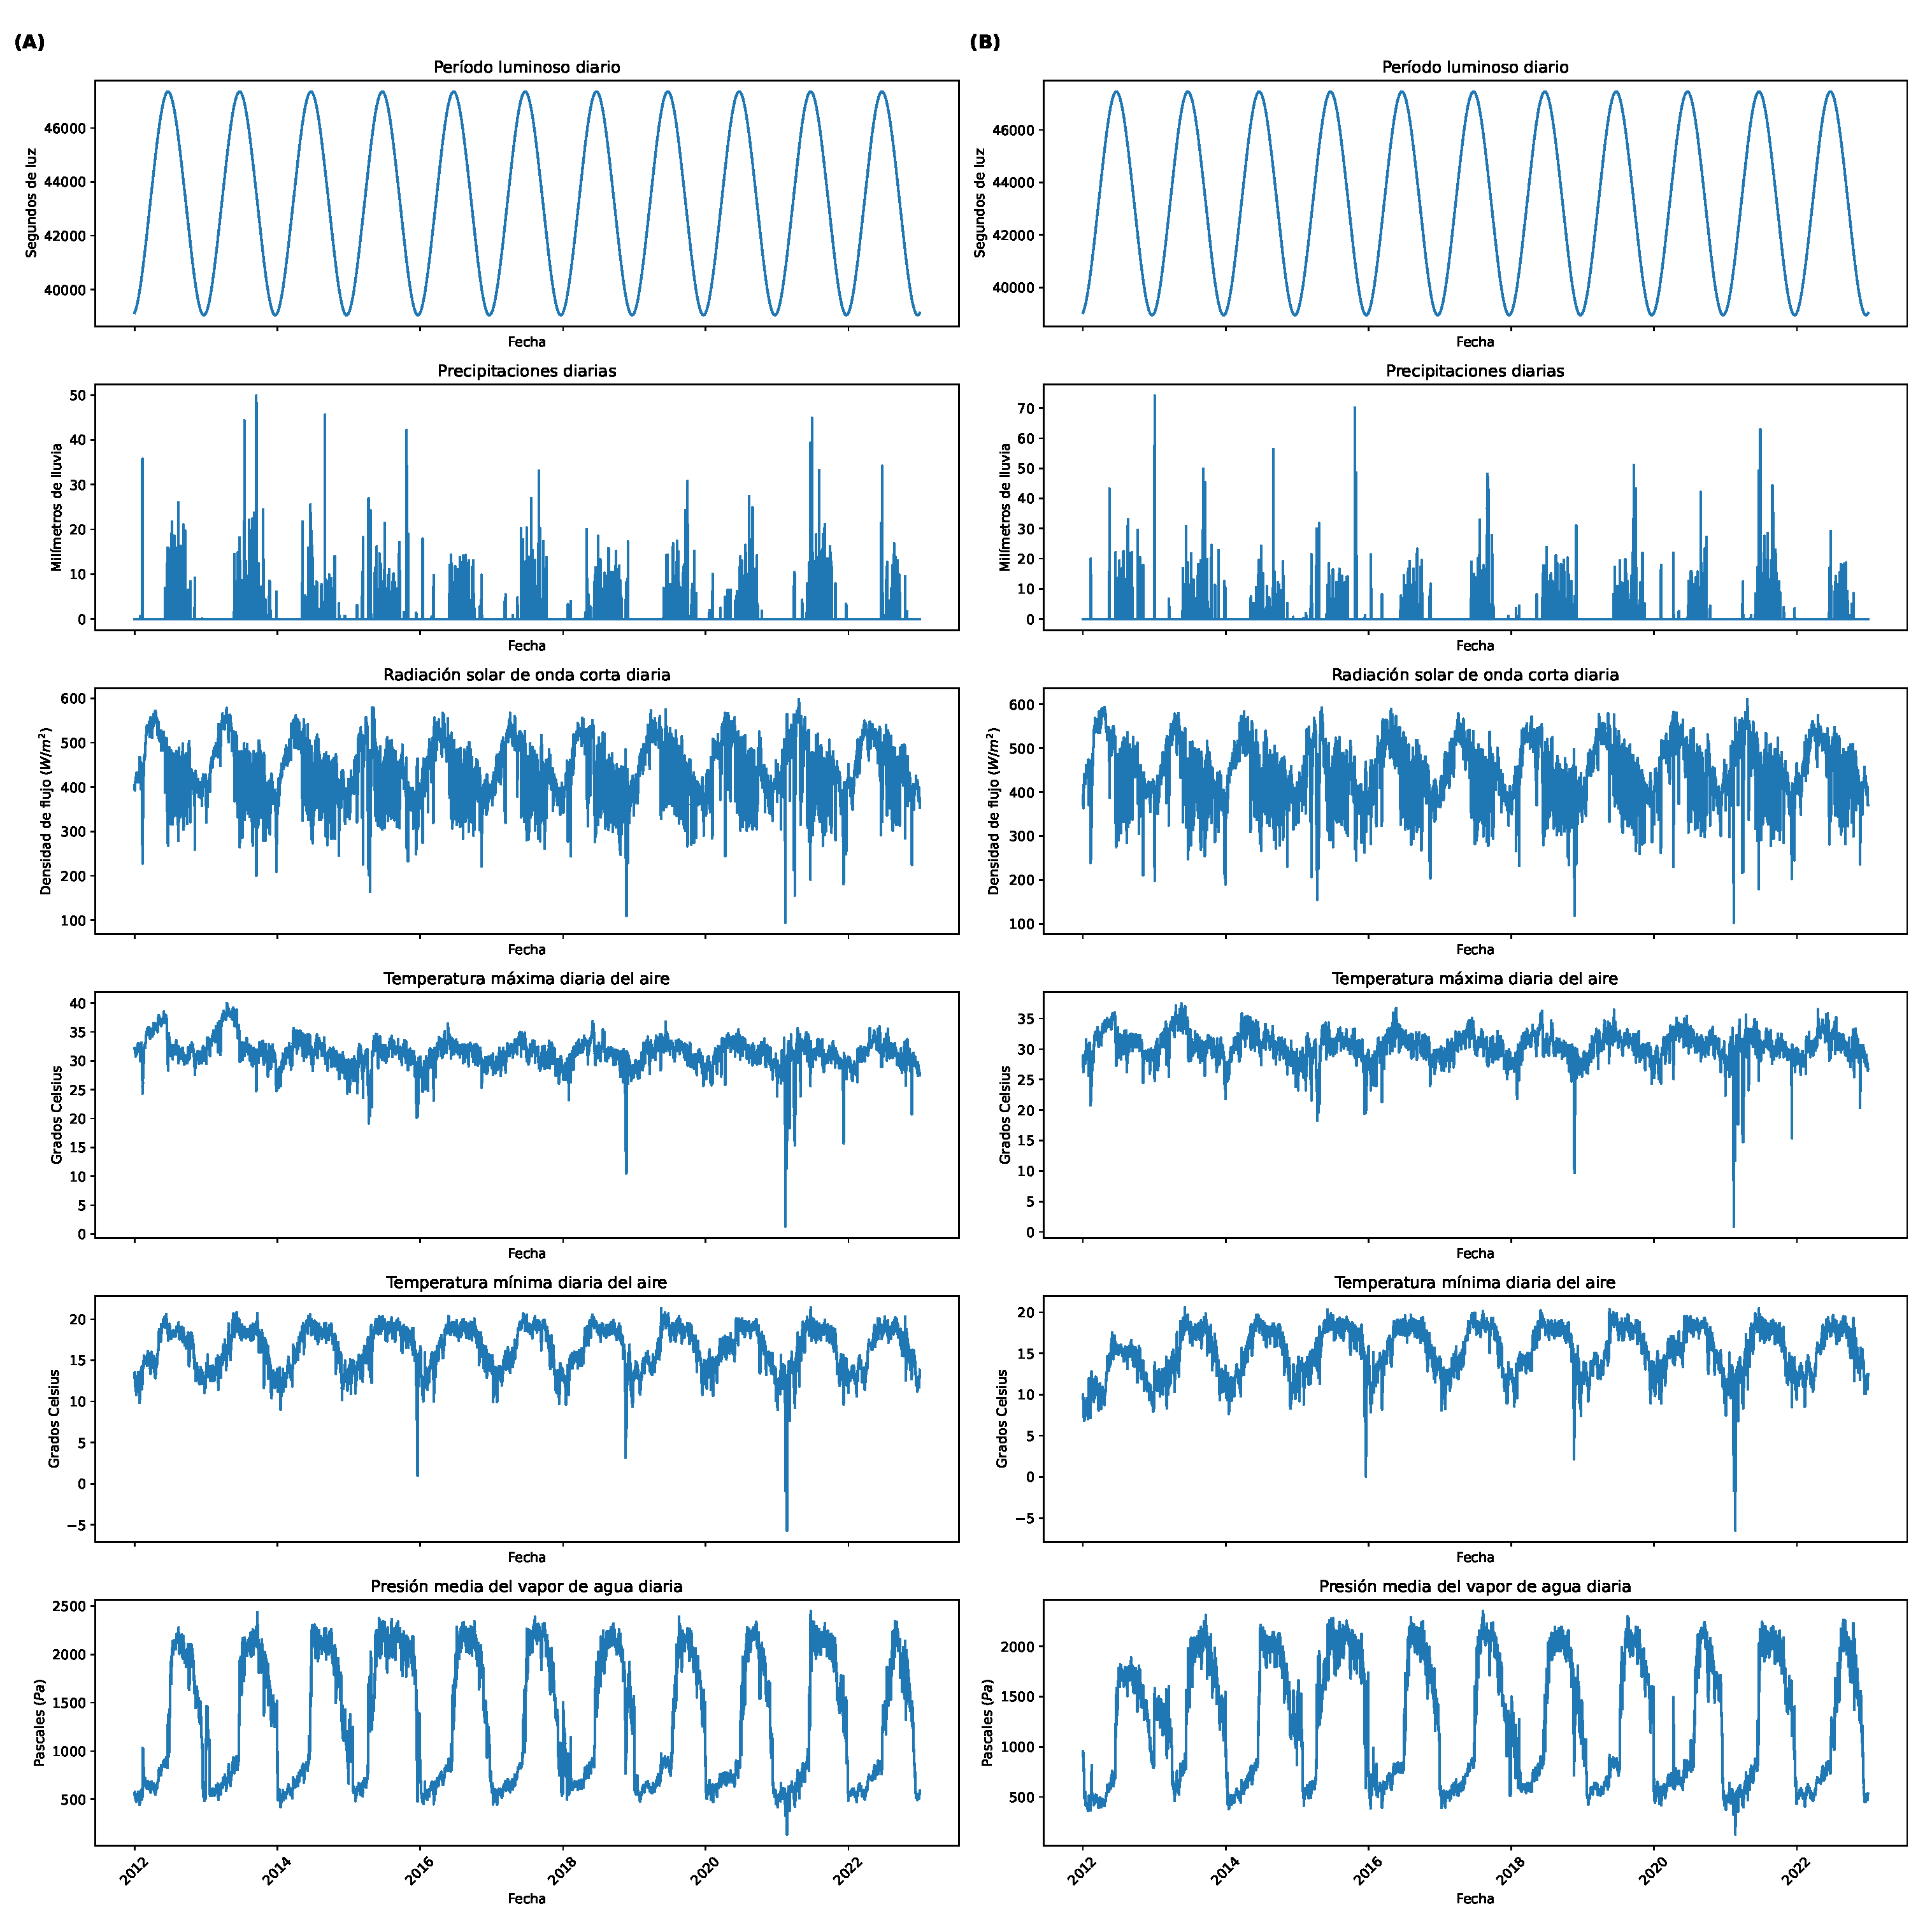
\includegraphics[width=1\linewidth]{Images/Meteorological_comparison.eps}
    \caption{Comparación de características meteorológicas históricas desde 2012 a 2022. La Figura \textbf{(A)} muestra los registros de la estación Pedernales de Tacámbaro, Michoacán; mientras que, la Figura \textbf{(B)} muestra los registros de la estación El Varal de Los Reyes, Michoacán. Figura construida a partir de los datos disponibles en \cite{Rodriguez-Moreno_2021}.}
    \label{fig:Meteorological_comparison}
\end{figure}


Estas variables influyen directamente en el proceso productivo del aguacate. La duración del período de luz influye en el tiempo disponible para el crecimiento de la planta, mientras que la cantidad de lluvia regula la disponibilidad de agua, esencial tanto para la planta como para las reservas de agua en el suelo. La radiación solar de onda corta proporciona la energía necesaria para la fotosíntesis a la par de calentar los tejidos de la planta y el suelo \cite{Jagadish_2021}, lo que a su vez afecta la actividad biológica y la disponibilidad de nutrientes.\\

Asimismo, las temperaturas máxima y mínima del aire inciden en la temperatura del suelo y, respecto a las plantas, intervienen en la floración y crecimiento \cite{Idso_1987}. La presión del vapor de agua, que está relacionada con la humedad en el aire, también impacta en la transpiración de la planta y en la retención de agua en el suelo.\\

Para complementar y formalizar el análisis visual que se desprende de la Figura \ref{fig:Meteorological_comparison}, se ejecutaron pruebas U de Mann--Whitney para analizar, variable por variable, la presencia de diferencias estadísticas entre las condiciones meteorológicas de Tacámbaro y Los Reyes. Lo anterior, a consecuencia de la falta de la hipótesis de normalidad, la cual fue probada a través de la prueba Shapiro--Wilk ($p<0.001$).\\


De las pruebas U de Mann--Whitney ejecutadas se concluye que hay diferencias estadísticamente significativas respecto a la radiación solar de onda corta ($p < 0.001$), temperatura máxima diaria del aire ($p < 0.001$), temperatura mínima diaria del aire ($p < 0.001$) y presión del vapor de agua ($p < 0.001$), ver Figura \ref{fig:Meteorological_statistical_comparison}. Estas diferencias podrían explicar el hecho de que el municipio de Los Reyes posee un mayor rendimiento por hectárea en comparación con el municipio de Tacámbaro, pero para estudiarlo se requerirá de un análisis más exhaustivo.\\

\begin{figure}[!ht]
    \centering
    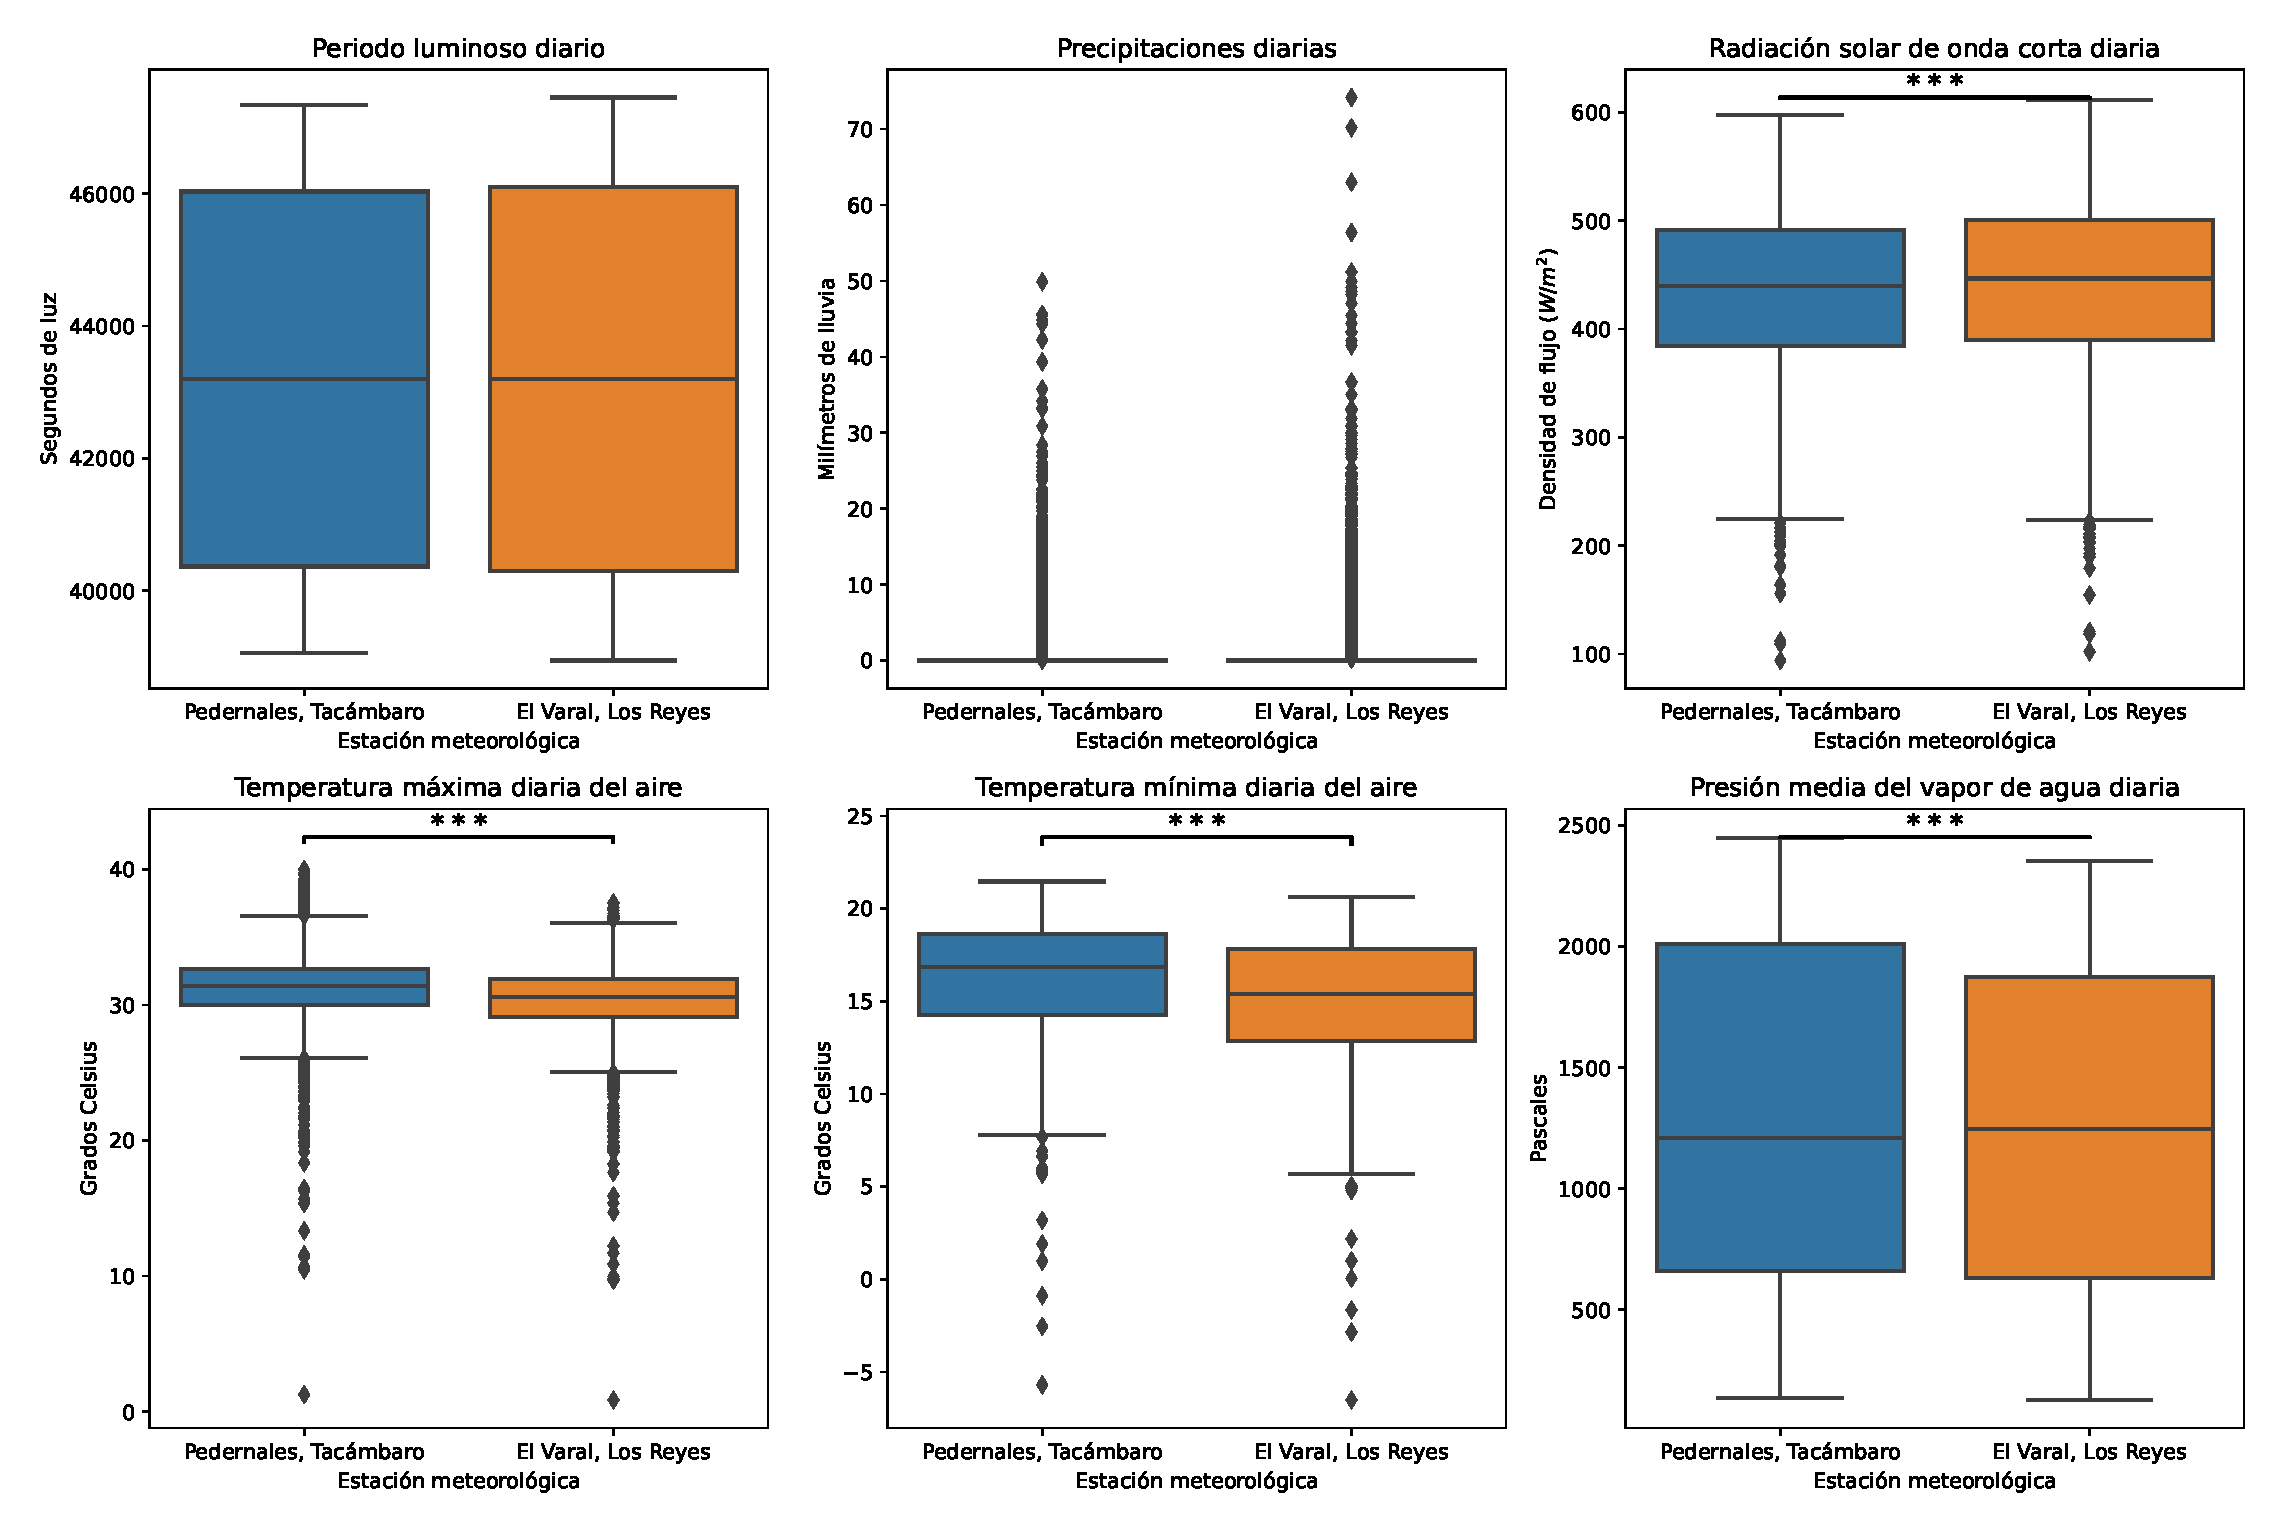
\includegraphics[width=1\linewidth]{Images/Meteorological_statistical_comparison.eps}
    \caption{Comparaciones estadísticas entre las características meteorológicas históricas desde 2012 a 2022. En azul se muestran los datos registrados por la estación Pedernales de Tacámbaro, Michoacán; mientras que, en naranja se muestra los registros de la estación El Varal de Los Reyes, Michoacán. Se aplicaron pruebas U de Mann--Whitney y la significancia estadística se denota a través de * ($p<0.05$), ** ($p<0.01$) y *** ($p<0.001$). Figura construida a partir de los datos disponibles en \cite{Rodriguez-Moreno_2021}.}
    \label{fig:Meteorological_statistical_comparison}
\end{figure}


Considerando tanto las características meteorológicas como los datos de producción que hemos analizado, ambas, de manera independiente. No obstante, ambas partes interactúan; por tanto, ahora estudiamos el efecto de tales características sobre los niveles de producción a través de medir la correlación entre ellas y su significancia estadística.\\


En consecuencia de la ausencia de la hipótesis de normalidad que se ha mencionado previamente, se calculó el coeficiente de correlación de Spearman, $\rho$, y su respectiva significancia estadística. La correlación de Spearman está definida para muestras de igual tamaño; por tanto, se calculó el promedio mensual de los datos meteorológicos dado que estos fueron registrados diariamente, desde el 1 de enero de 2012 hasta el 31 de diciembre de 2022; mientras que los datos de producción se registran con una frecuencia mensual, desde el 1 de enero de 2018 hasta el 31 de enero de 2025. Además, se consideró el periodo en donde ambos registros se intersecan en el tiempo; es decir, de enero de 2018 a diciembre de 2022.\\

Con el planteamiento anterior, para cada una de las variables de producción y rendimiento de aguacates se calculó su correlación de Spearman con las variables meteorológicas. Y para minimizar el riesgo de falsos positivos, se aplicó la corrección de Bonferroni, evitando así concluir erróneamente la existencia de una correlación estadísticamente significativa \cite{Curtin_1998}.\\

En la Figura \ref{fig:CorrelacionProduccionMensual} se presentan los resultados asociados a la producción mensual de aguacates. Respecto a Tacámbaro, la producción mensual tiene una correlación negativa estadísticamente significativa con el periodo luminoso ($\rho =-0.49$, $p < 0.001$), la radiación solar de onda corta ($\rho =-0.51$, $p<0.001$) y la temperatura máxima del aire ($\rho =-0.5$, $p<0.001$), ver Figura \ref{fig:CorrelacionProduccionMensual_Tacámbaro}. Por otra parte, respecto a Los Reyes, la producción mensual tiene una correlación negativa estadísticamente significativa con el periodo luminoso ($\rho =-0.42$, $p < 0.01$) y la temperatura mínima del aire ($\rho =-0.45$, $p<0.01$), ver Figura \ref{fig:CorrelacionProduccionMensual_Los Reyes}.\\

\begin{figure}[ht]
\centering
\subfloat[Tacámbaro]{\label{fig:CorrelacionProduccionMensual_Tacámbaro}
\centering
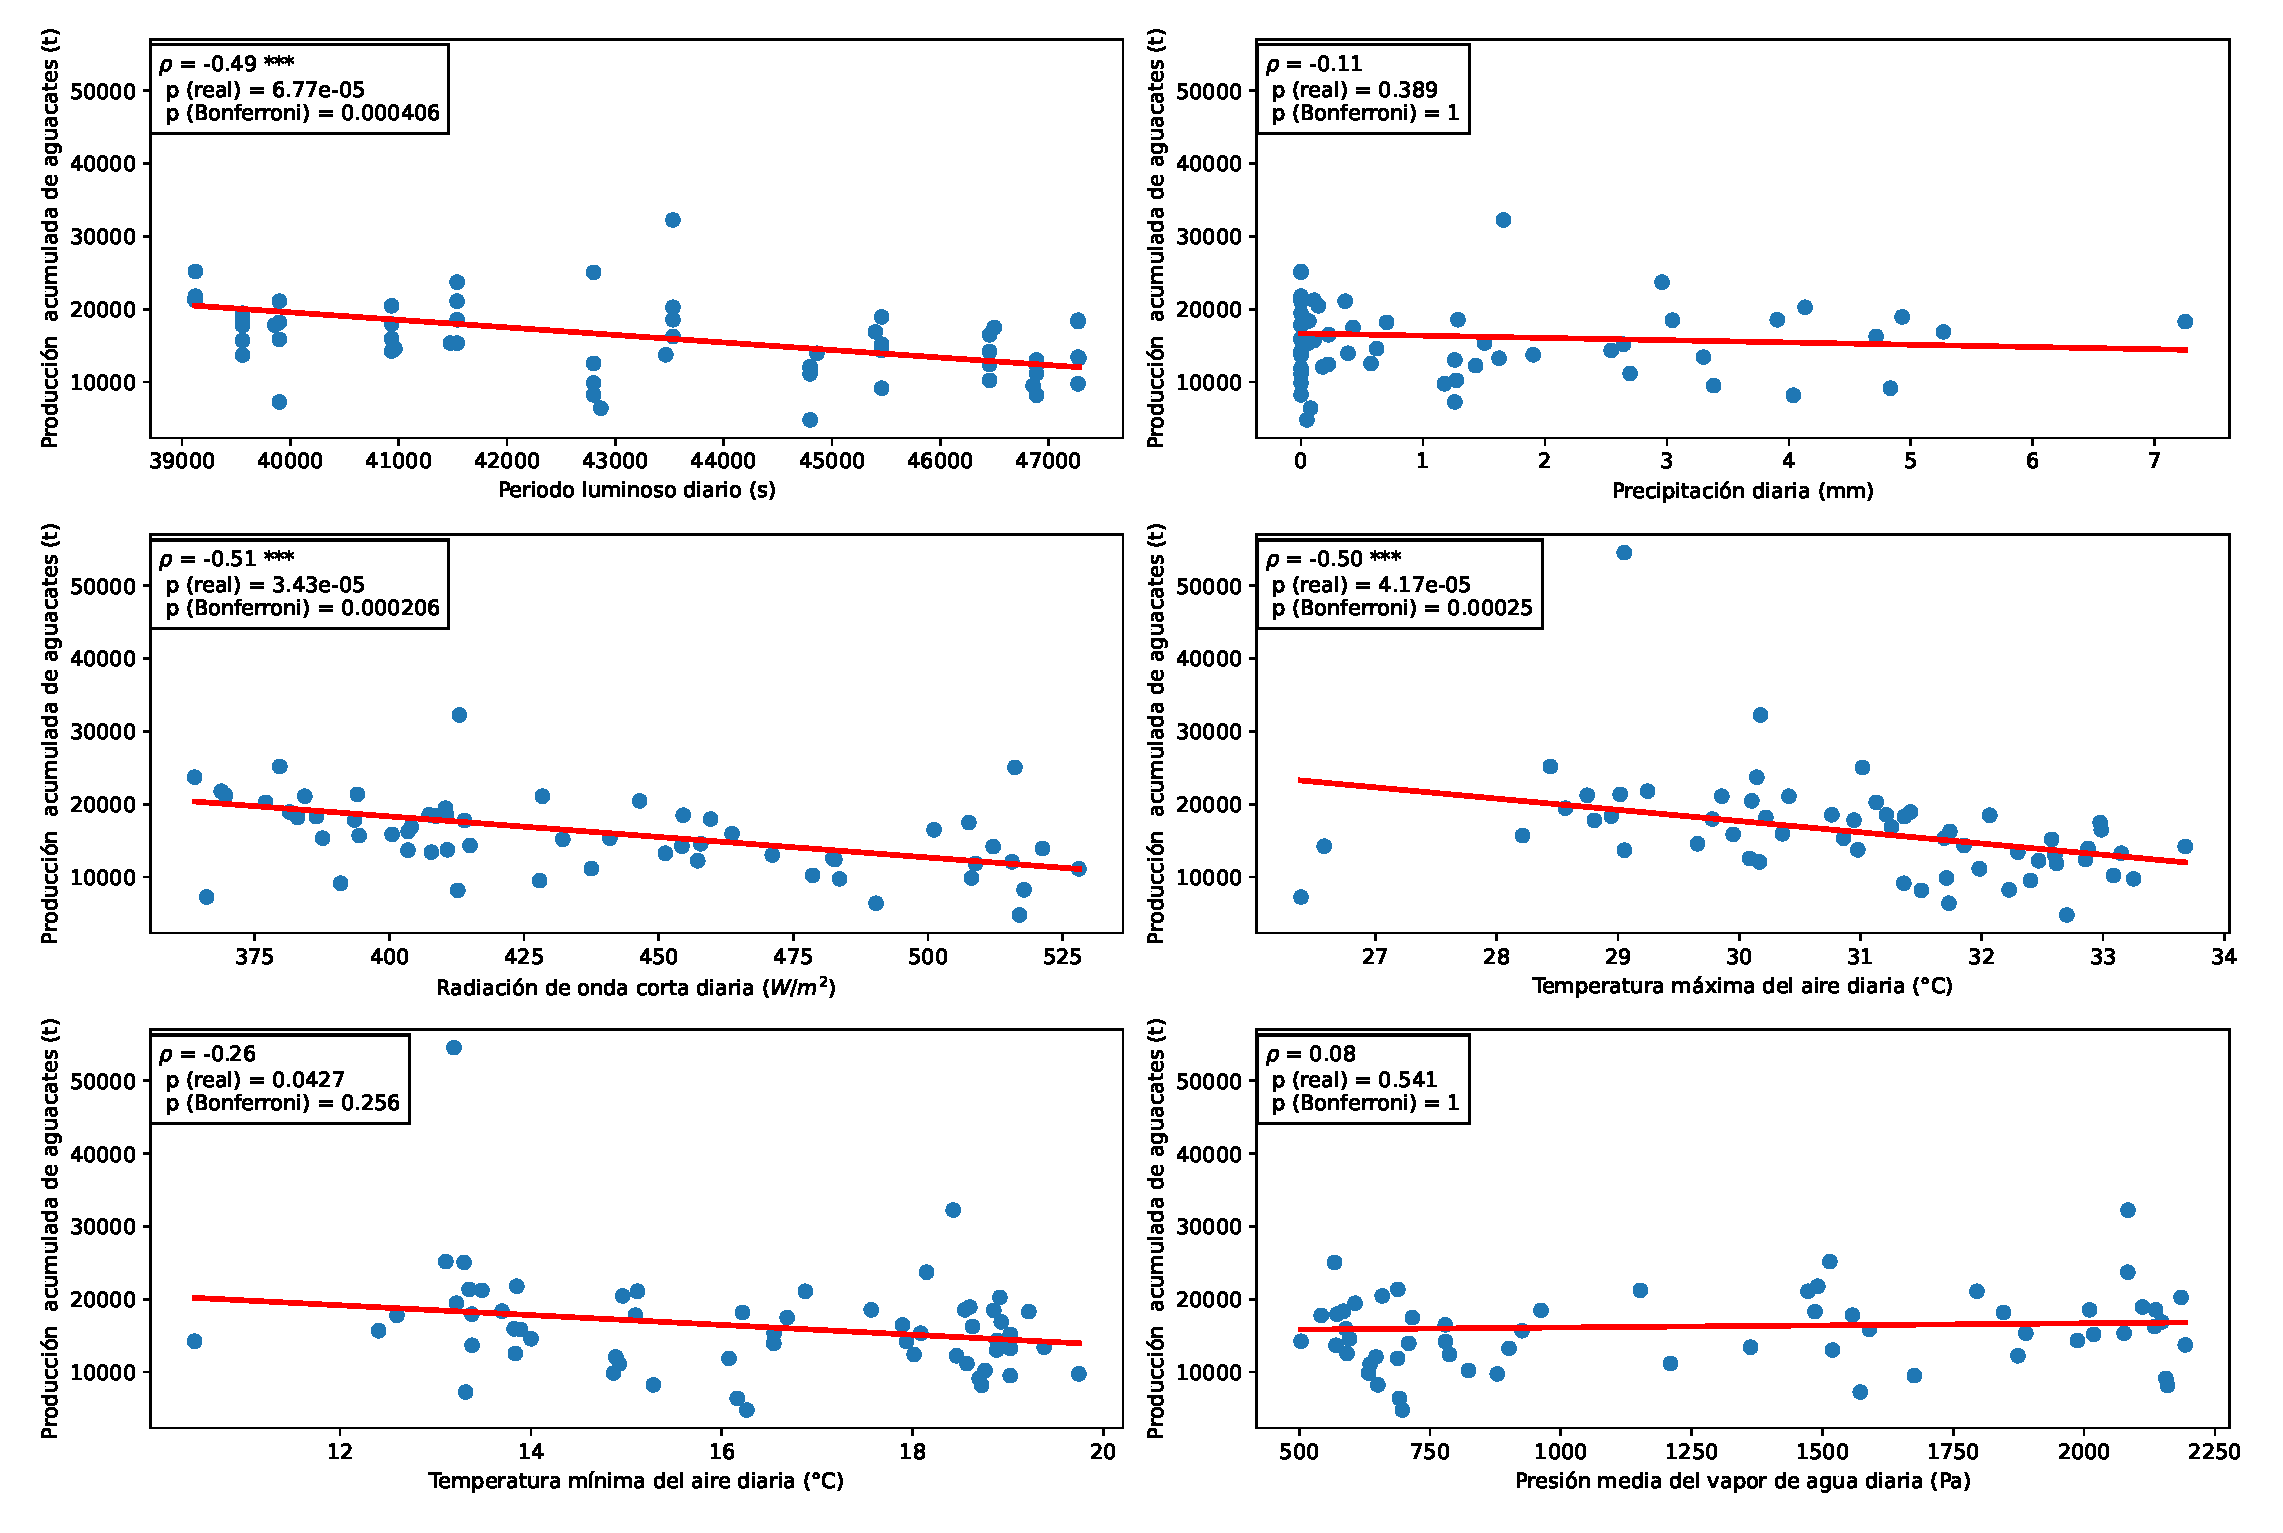
\includegraphics[width=0.8\linewidth]{Images/Effect_on_monthly_production_Tacambaro.eps}
}
%no space
\hfill
\subfloat[Los Reyes]{\label{fig:CorrelacionProduccionMensual_Los Reyes}
\centering
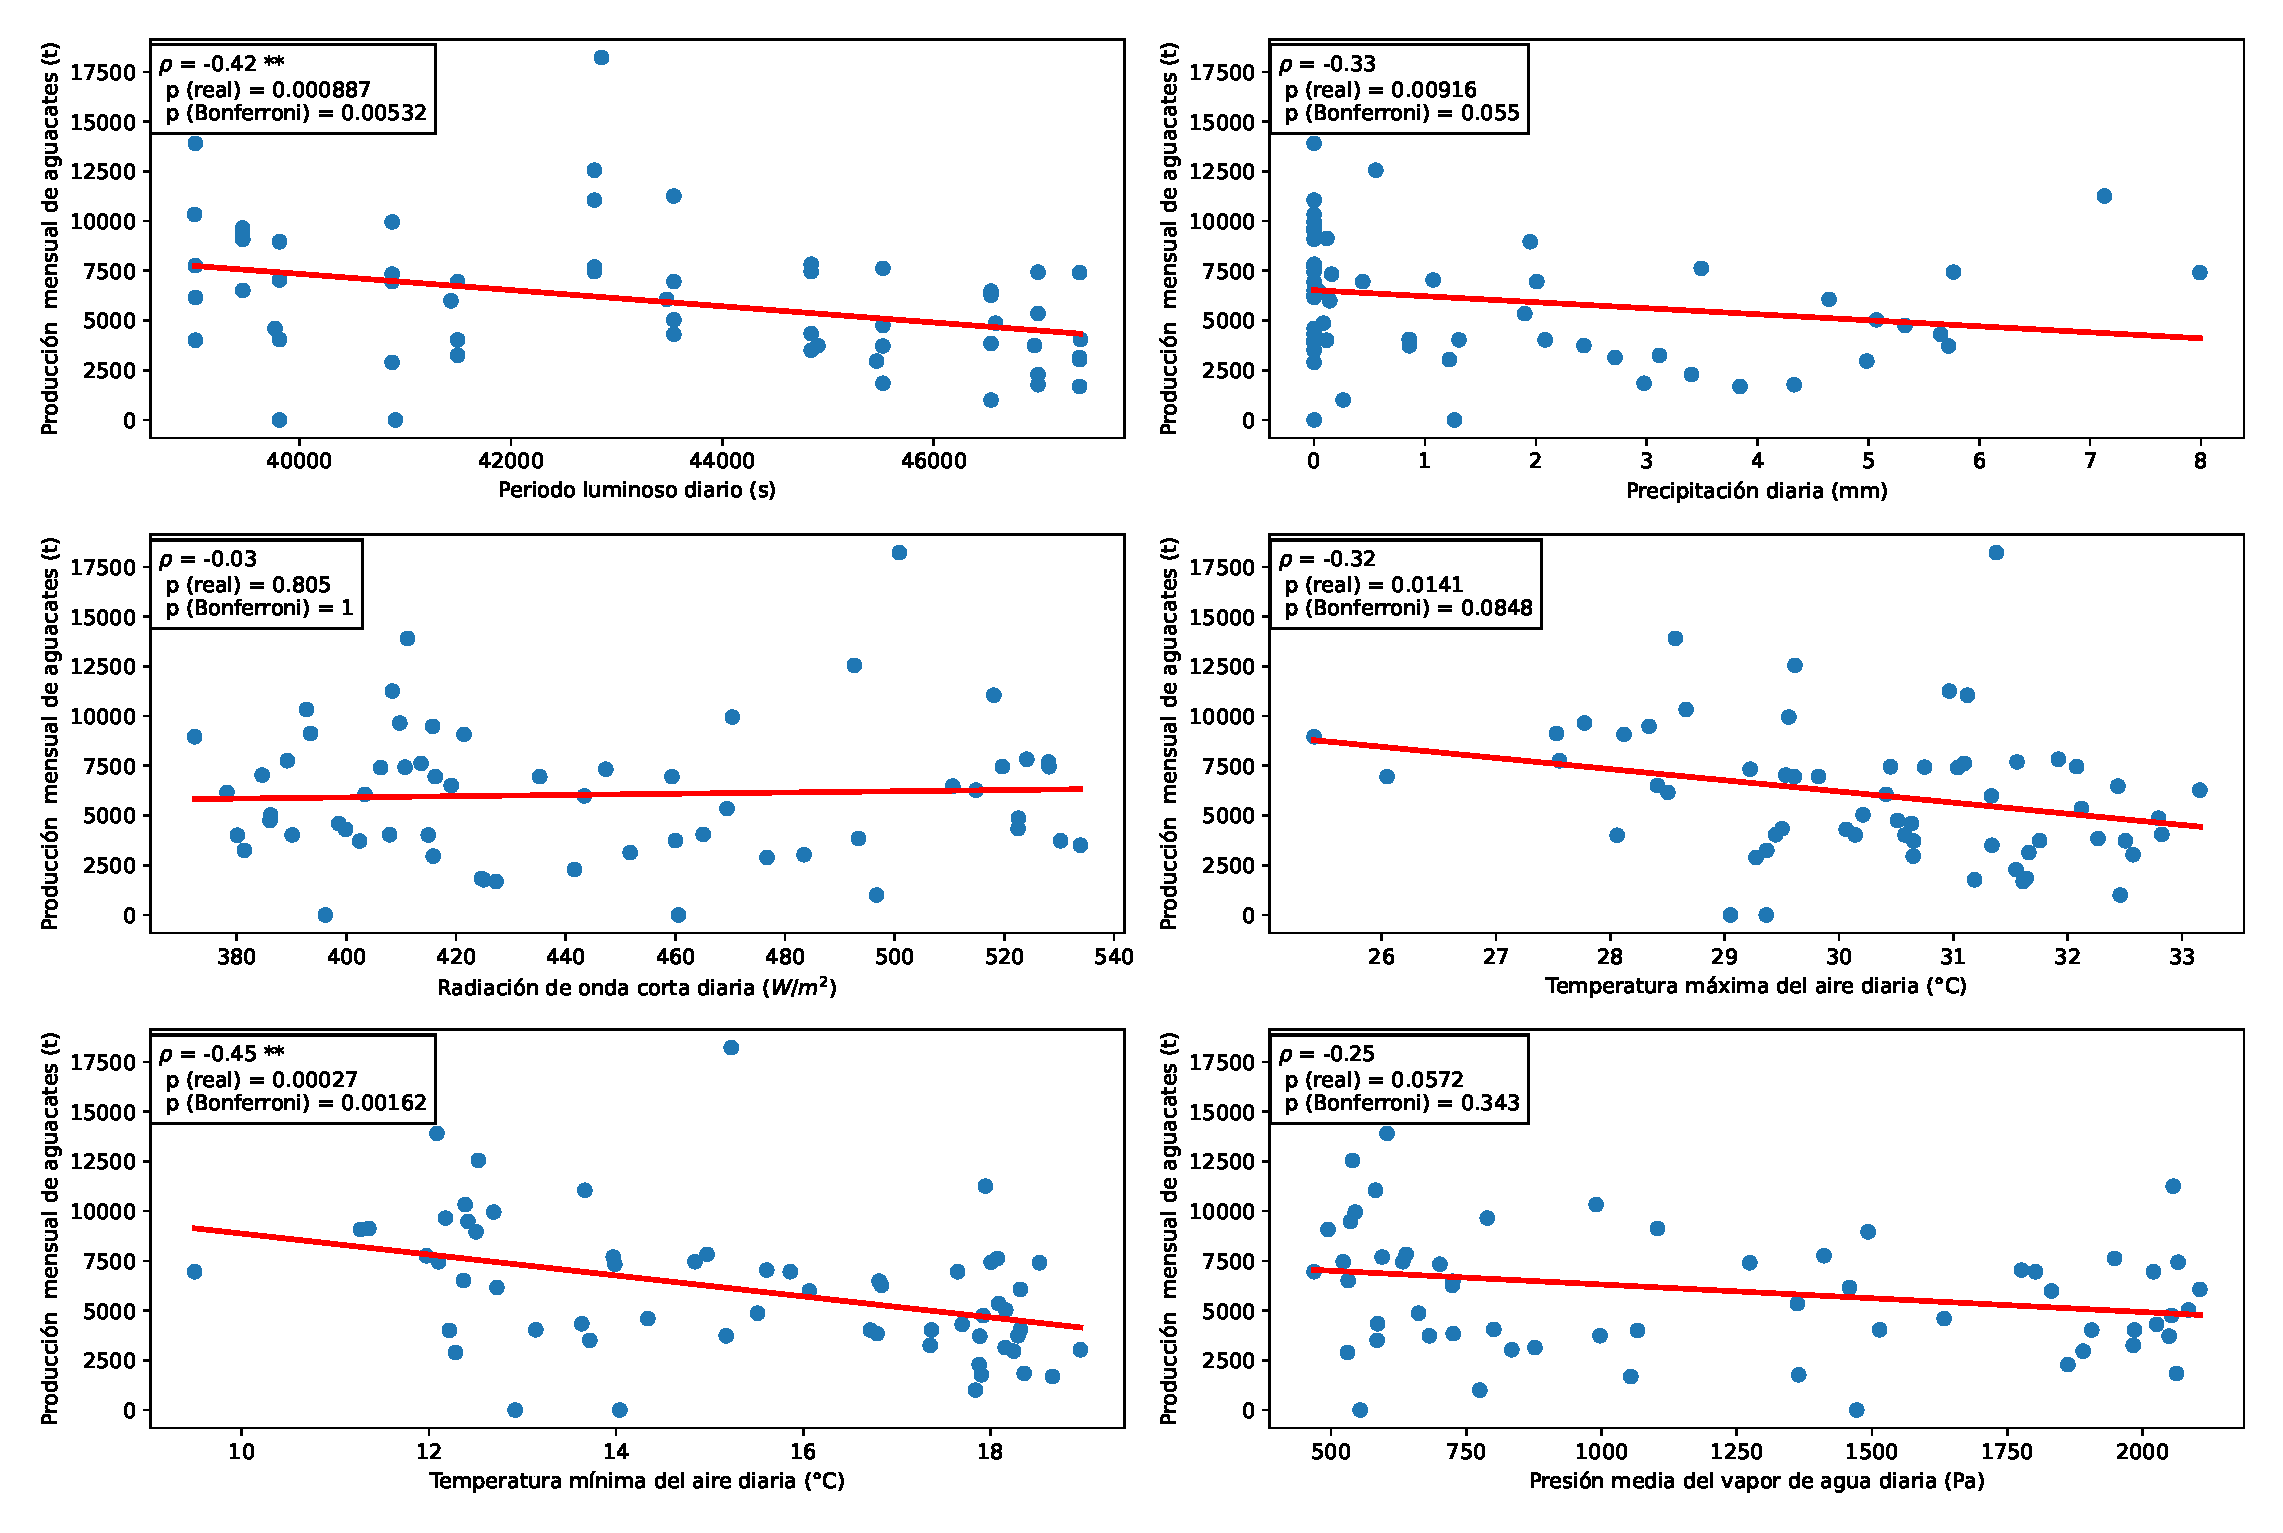
\includegraphics[width=0.8\linewidth]{Images/Effect_on_monthly_production_LosReyes.eps}
}
\caption{Análisis de correlación entre las variables meteorológicas y la producción mensual de aguacates. La Figura \ref{fig:CorrelacionProduccionMensual_Tacámbaro} ilustra los resultados obtenidos para Tacámbaro; mientras que, la Figura \ref{fig:CorrelacionProduccionMensual_Los Reyes} muestra lo obtenido para Los Reyes. Se aplicaron correlaciones de Spearman con corrección de Bonferroni y su significancia estadística se denota a través de * ($p<0.05$), ** ($p<0.01$) y *** ($p<0.001$). Figura construida a partir de los datos disponibles en \cite{AvanceSiembrasCosechas} y \cite{Rodriguez-Moreno_2021}.}
\label{fig:CorrelacionProduccionMensual}
\end{figure}


En la Figura \ref{fig:CorrelacionProduccionAcumulada} se muestran los resultados referentes a la producción acumulada de aguacates. Respecto a Tacámbaro, la producción acumulada tiene una correlación negativa estadísticamente significativa con la radiación de onda corta ($\rho =-0.6$, $p<0.001$) y una correlación positiva estadísticamente significativa con la presión del vapor de agua ($\rho =0.69$, $p<0.001$), ver Figura \ref{fig:CorrelacionProduccionAcumulada_Tacambaro}. Similarmente, respecto a Los Reyes, la producción acumulada tiene una correlación negativa estadísticamente significativa con la radiación de onda corta ($\rho =-0.53$, $p<0.001$) y una correlación positiva estadísticamente significativa con la presión del vapor de agua ($\rho =0.65$, $p<0.001$), ver Figura \ref{fig:CorrelacionProduccionAcumulada_Los Reyes}.\\

\begin{figure}[ht]
\centering
\subfloat[Tacámbaro]{\label{fig:CorrelacionProduccionAcumulada_Tacambaro}
\centering
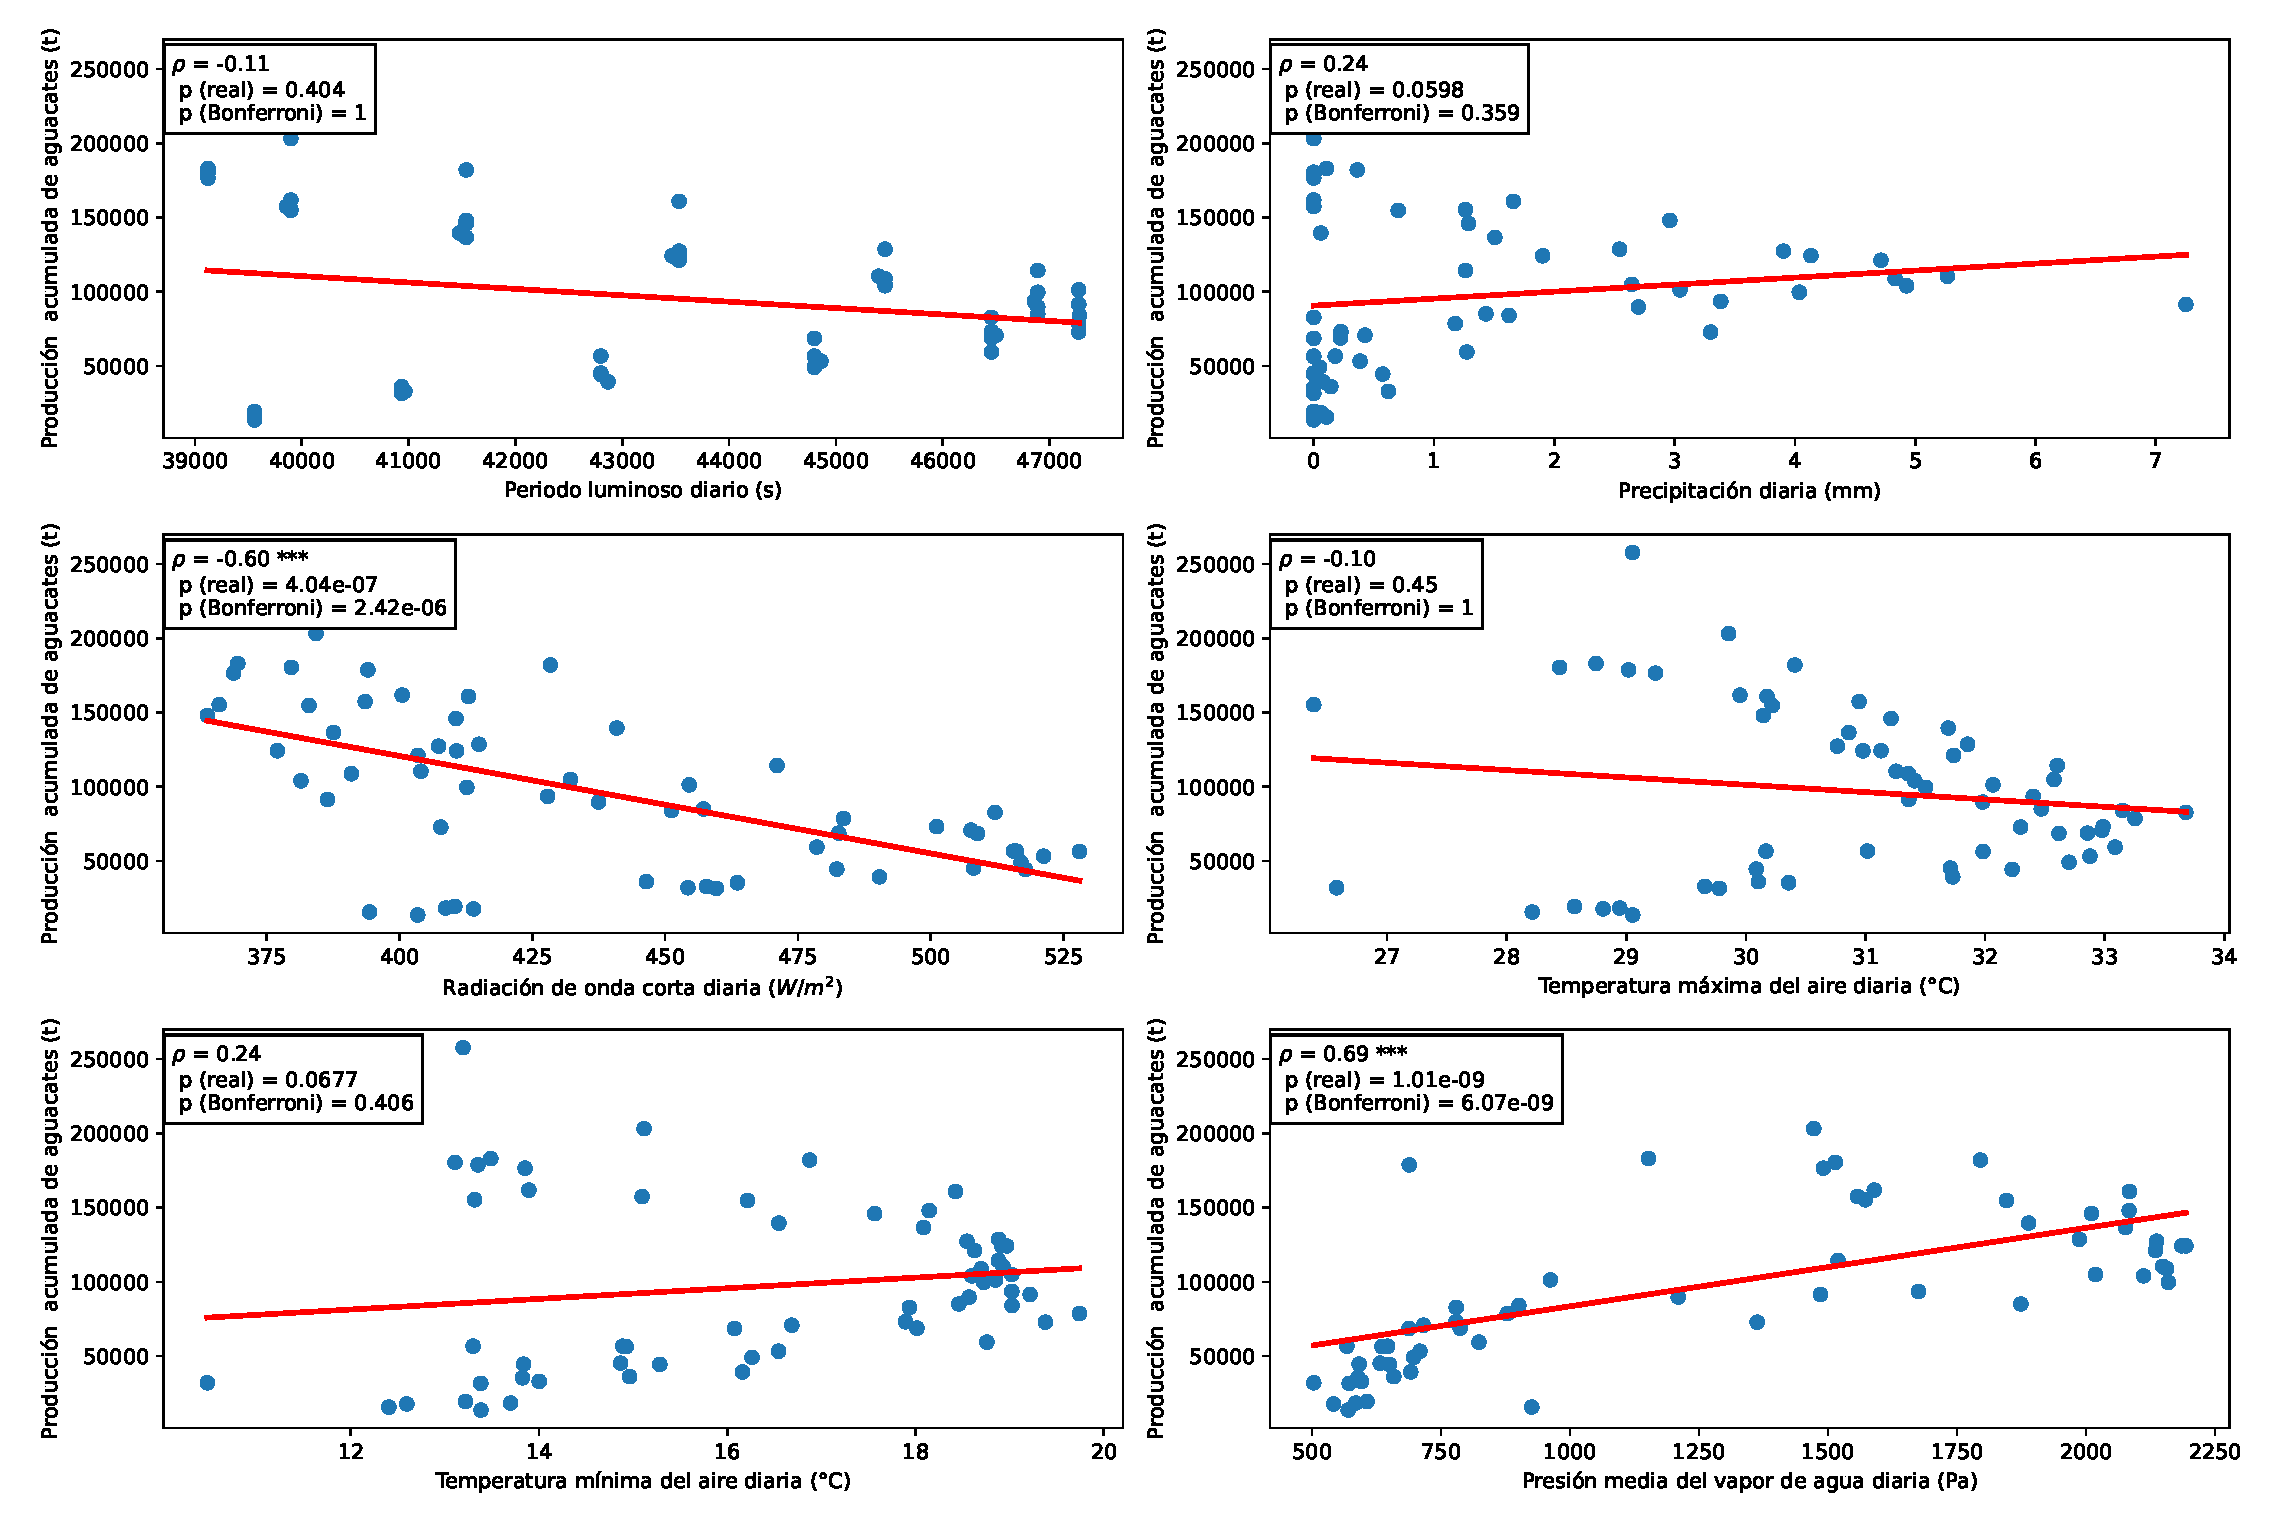
\includegraphics[width=0.8\linewidth]{Images/Effect_on_cumulative_production_Tacambaro.eps}
}
%no space
\hfill
\subfloat[Los Reyes]{\label{fig:CorrelacionProduccionAcumulada_Los Reyes}
\centering
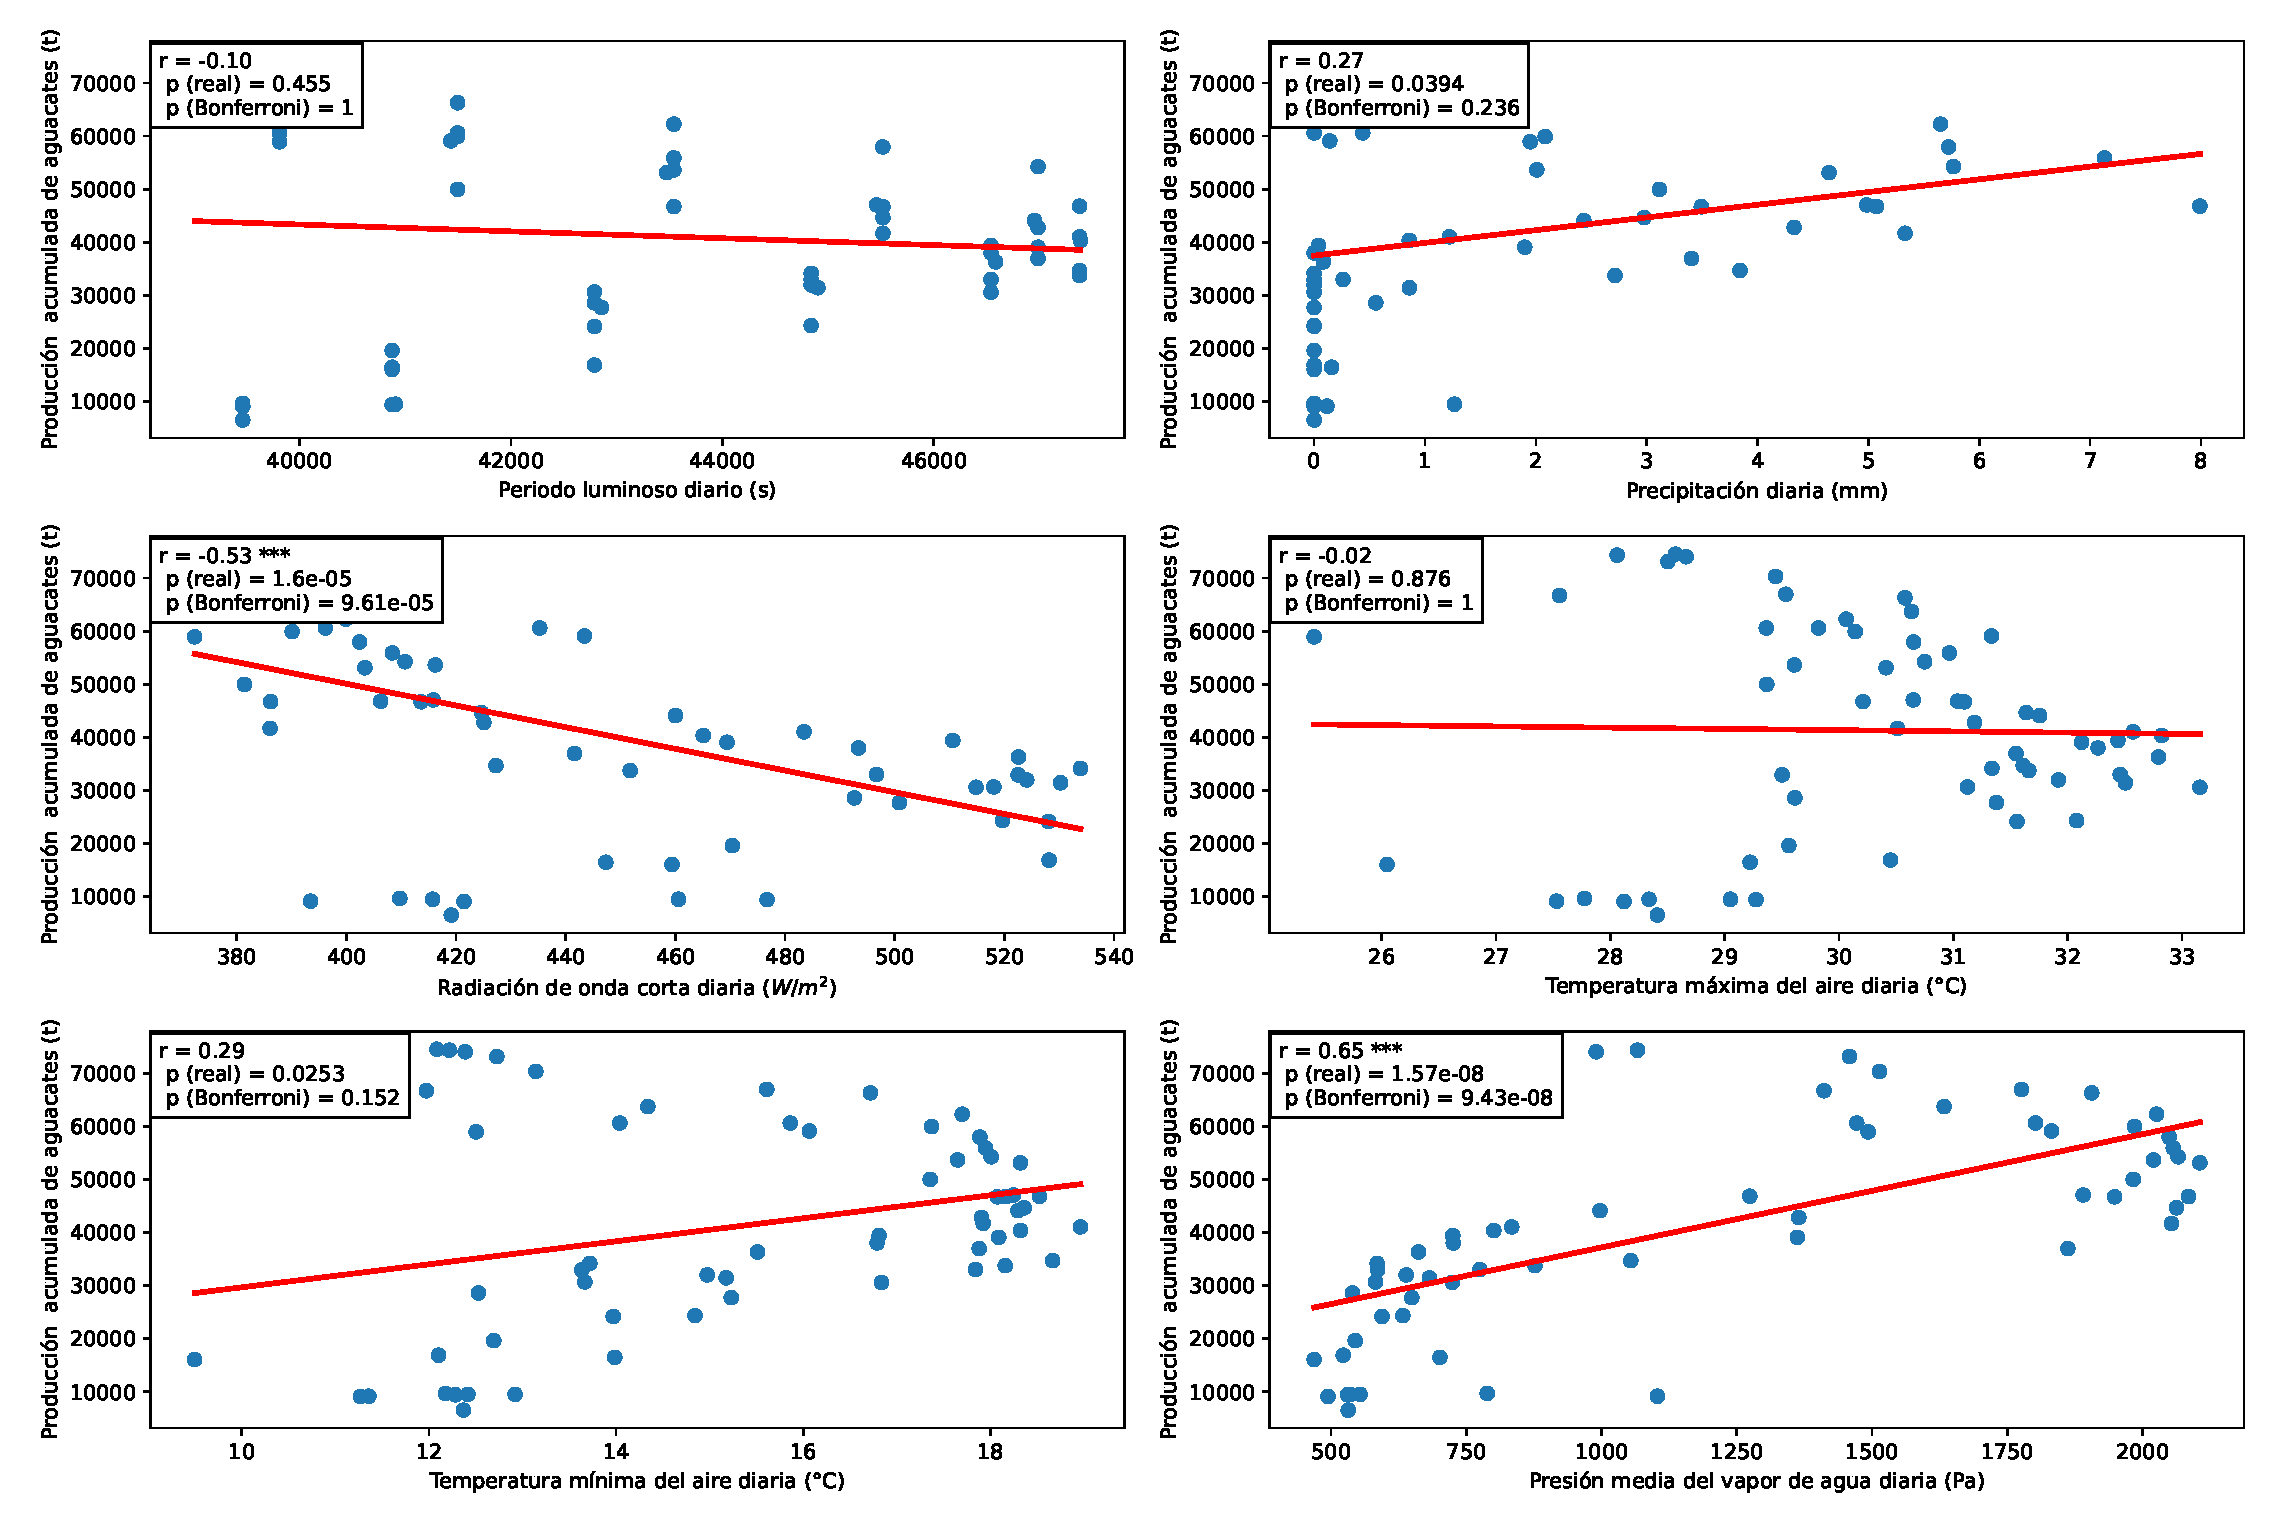
\includegraphics[width=0.8\linewidth]{Images/Effect_on_cumulative_production_LosReyes.eps}
}
\caption{Análisis de correlación entre las variables meteorológicas y la producción acumulada de aguacates. La Figura \ref{fig:CorrelacionProduccionAcumulada_Tacambaro} ilustra los resultados obtenidos para Tacámbaro; mientras que, la Figura \ref{fig:CorrelacionProduccionAcumulada_Los Reyes} muestra lo obtenido para Los Reyes. Se aplicaron correlaciones de Spearman con corrección de Bonferroni y su significancia estadística se denota a través de * ($p<0.05$), ** ($p<0.01$) y *** ($p<0.001$). Figura construida a partir de los datos disponibles en \cite{AvanceSiembrasCosechas} y \cite{Rodriguez-Moreno_2021}.}
\label{fig:CorrelacionProduccionAcumulada}
\end{figure}




La Figura \ref{fig:CorrelacionRendimientoMensual} ilustra las correlaciones referentes al rendimiento mensual por hectárea de aguacates. Respecto a Tacámbaro, el rendimiento mensual tiene una correlación negativa estadísticamente significativa con el periodo luminoso ($\rho =-0.51$, $p<0.001$), la radiación de onda corta ($\rho =-0.57$, $p<0.001$) y con la temperatura máxima del aire ($\rho = -0.51$, $p<0.001$), ver Figura \ref{fig:CorrelacionRendimientoMensual_Tacambaro}. Por otra parte, respecto a Los Reyes, el rendimiento mensual tiene una correlación negativa estadísticamente significativa con el periodo luminoso ($\rho =-0.43$, $p<0.01$) y la temperatura mínima del aire  ($\rho =-0.46$, $p<0.01$), ver Figura \ref{fig:CorrelacionRendimientoMensual_Los Reyes}.\\


\begin{figure}[ht]
\centering
\subfloat[Tacámbaro]{\label{fig:CorrelacionRendimientoMensual_Tacambaro}
\centering
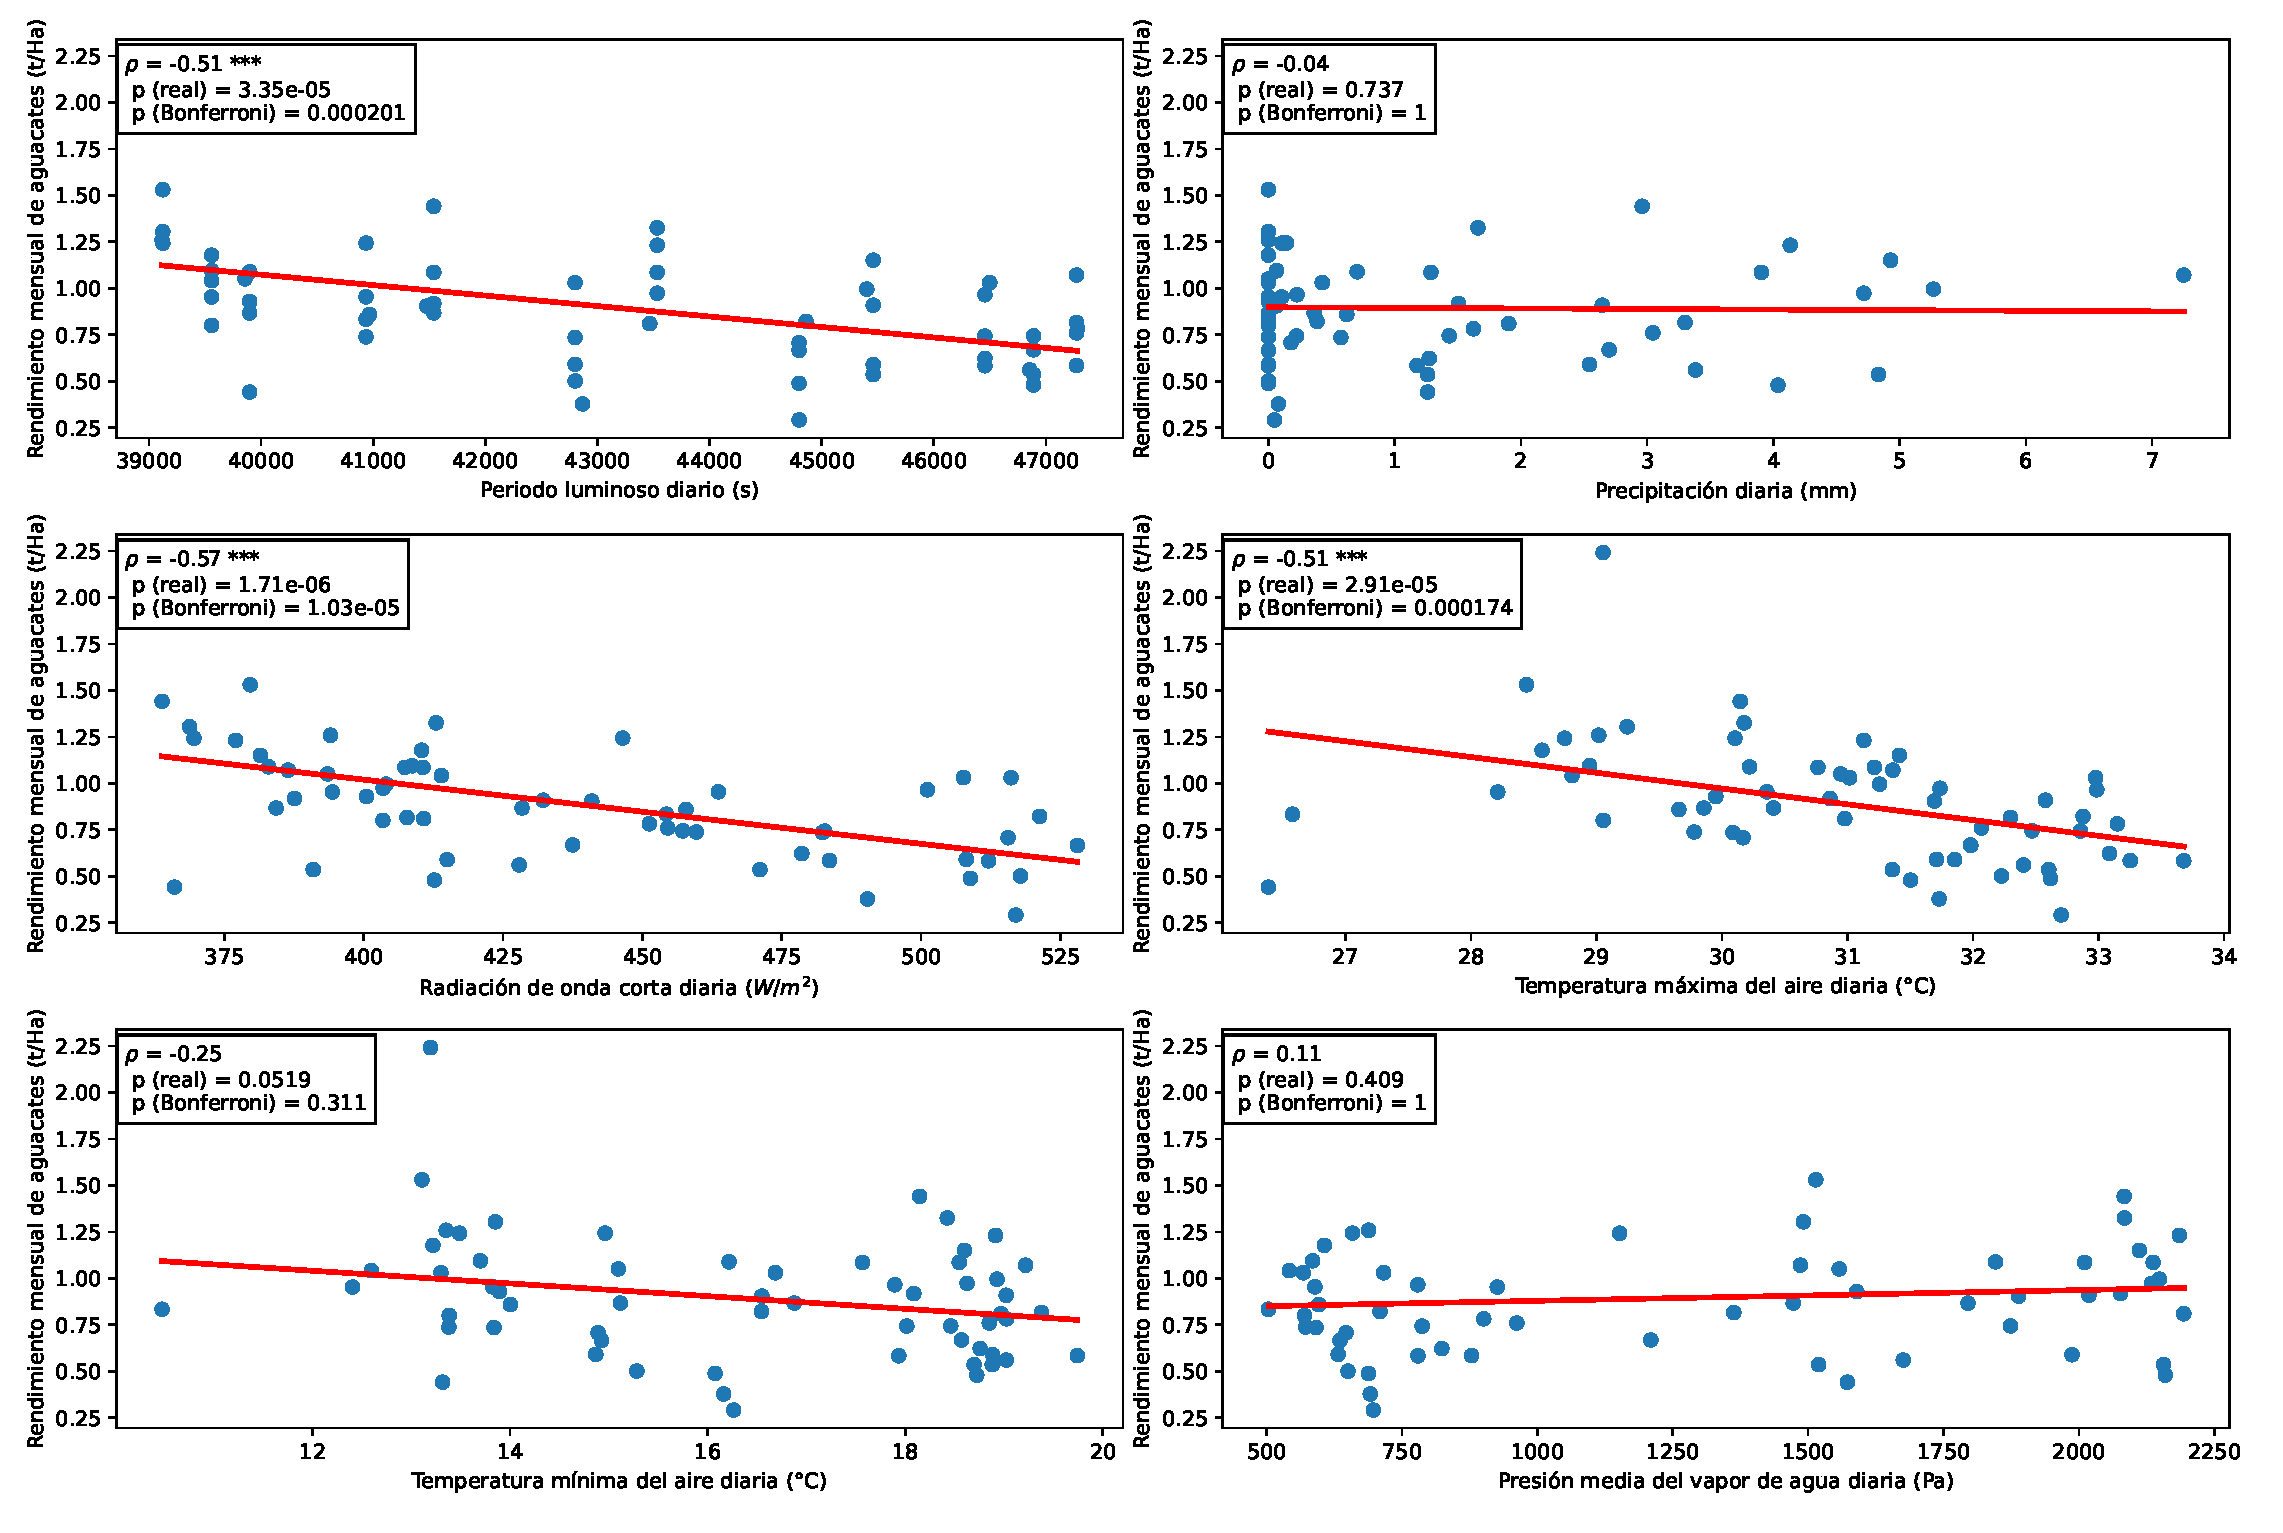
\includegraphics[width=0.8\linewidth]{Images/Effect_on_MonthlyPerformance_Tacambaro.eps}
}
%no space
\hfill
\subfloat[Los Reyes]{\label{fig:CorrelacionRendimientoMensual_Los Reyes}
\centering
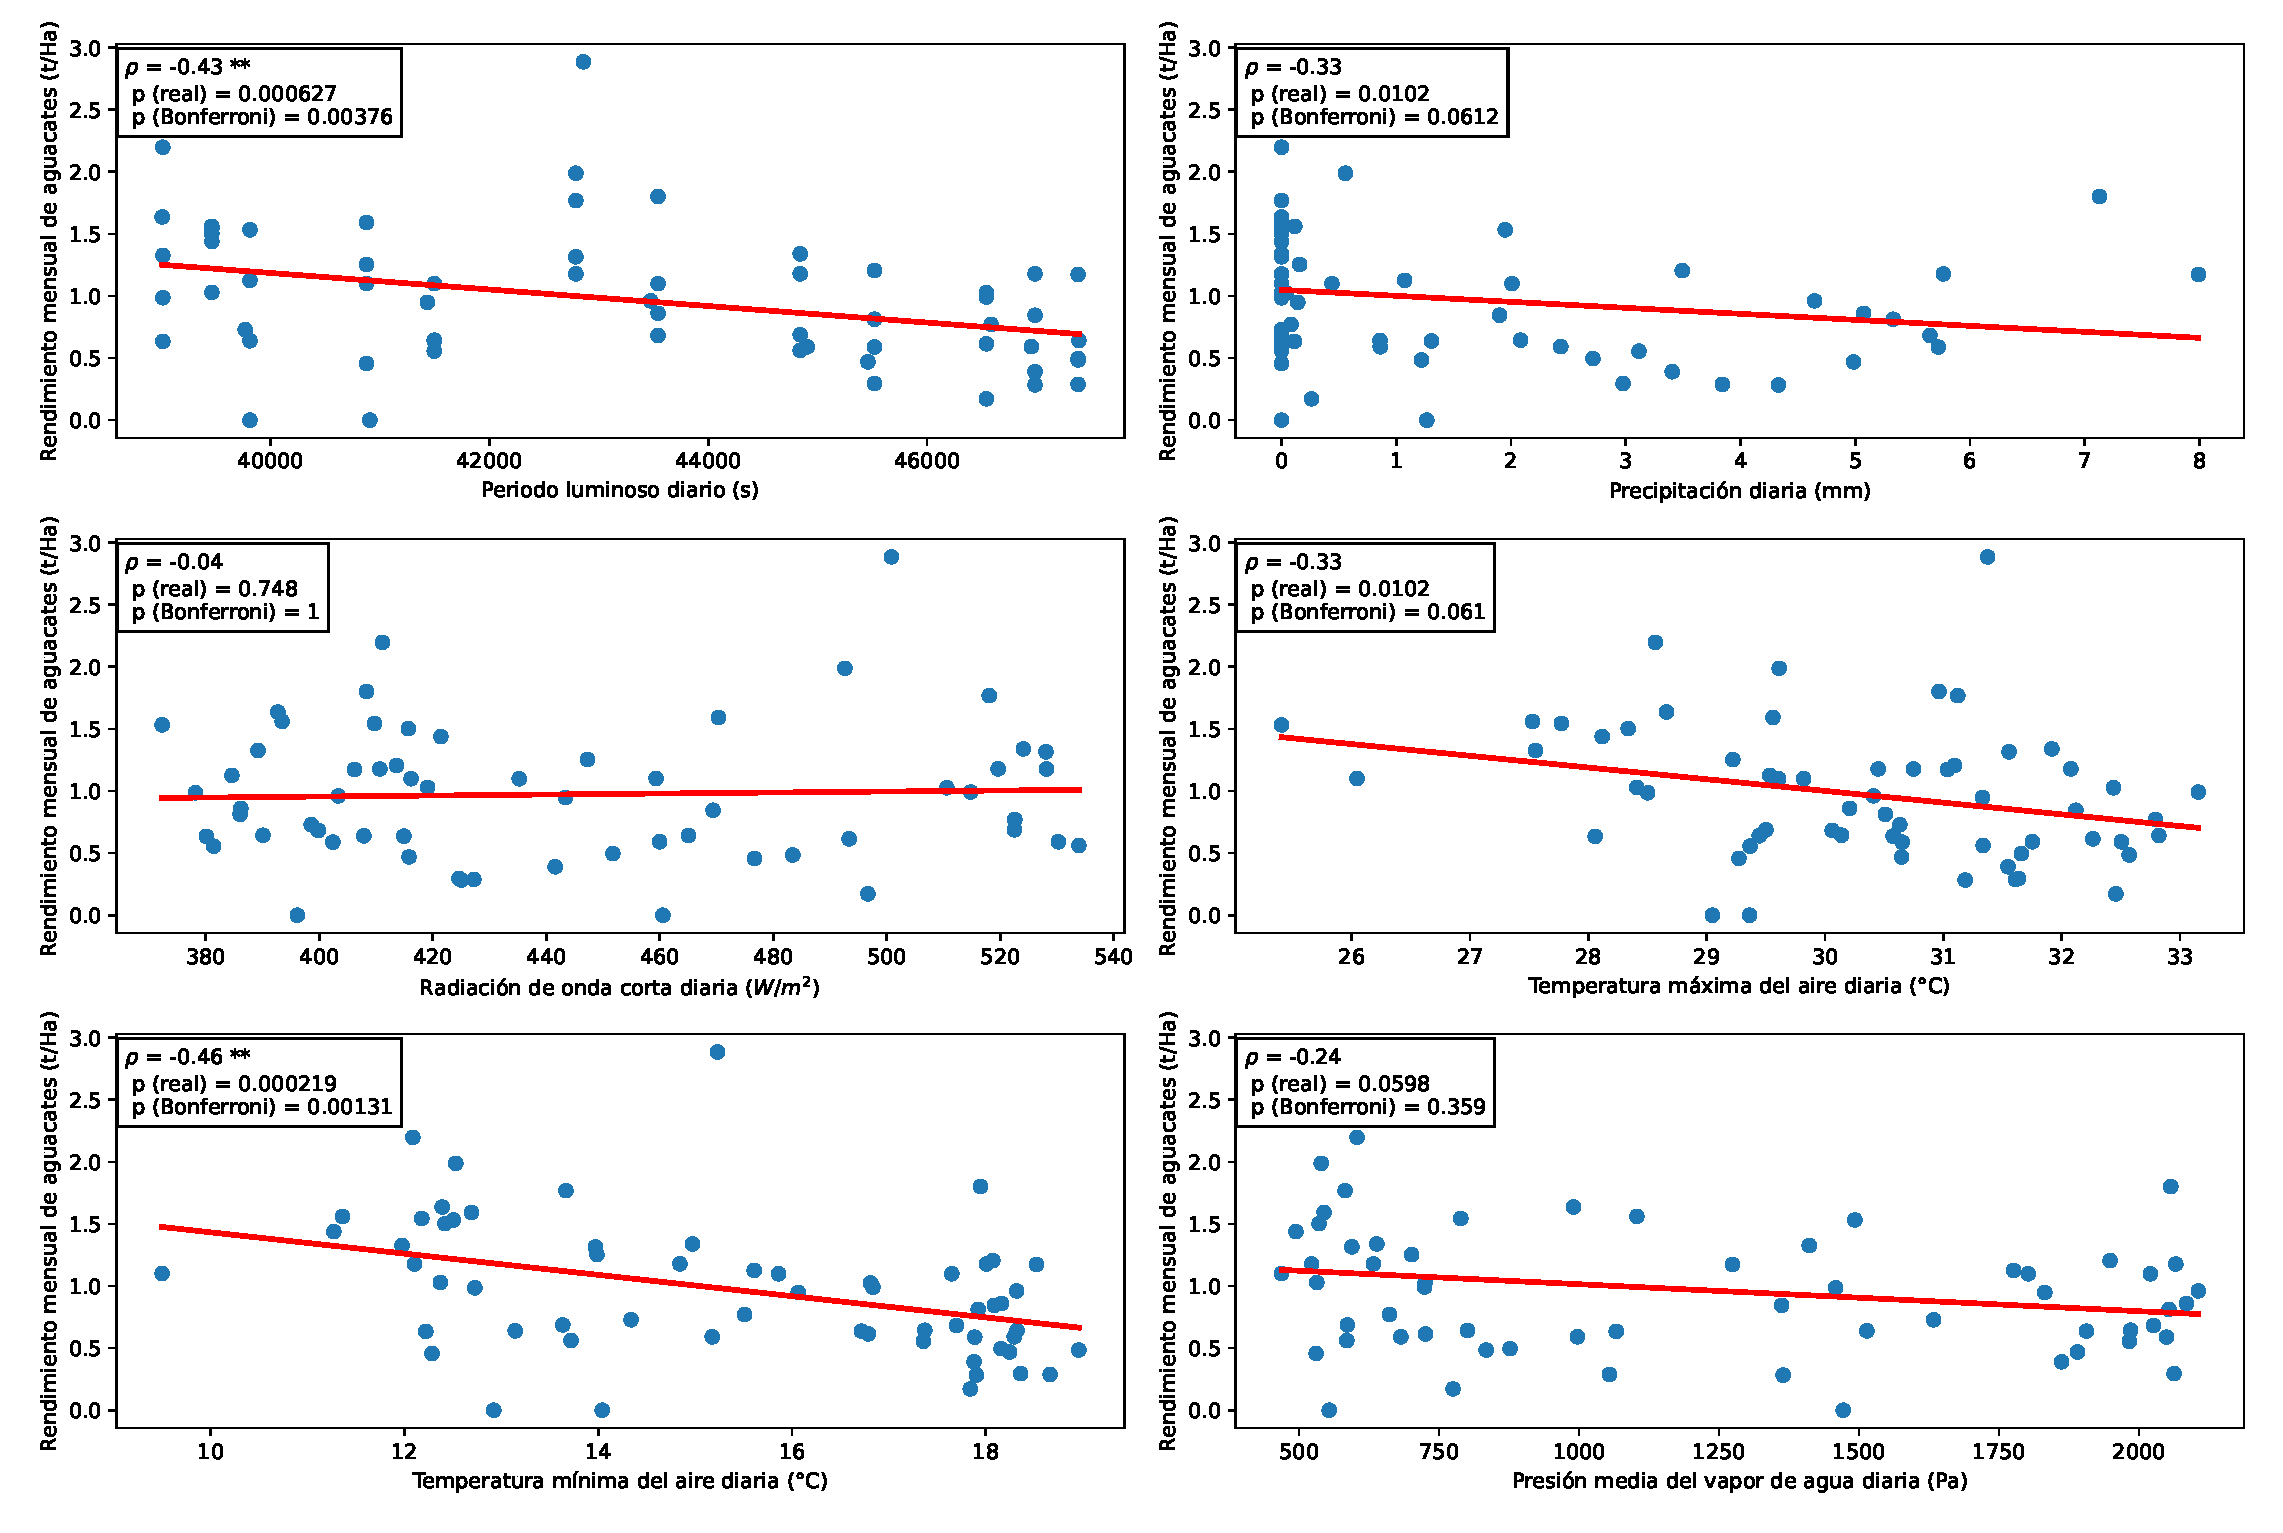
\includegraphics[width=0.8\linewidth]{Images/Effect_on_MonthlyPerformance_LosReyes.eps}
}
\caption{Análisis de correlación entre las variables meteorológicas y el rendimiento mensual de aguacates. La Figura \ref{fig:CorrelacionProduccionAcumulada_Tacambaro} ilustra los resultados obtenidos para Tacámbaro; mientras que, la Figura \ref{fig:CorrelacionProduccionAcumulada_Los Reyes} muestra lo obtenido para Los Reyes. Se aplicaron correlaciones de Spearman con corrección de Bonferroni y su significancia estadística se denota a través de * ($p<0.05$), ** ($p<0.01$) y *** ($p<0.001$). Figura construida a partir de los datos disponibles en \cite{AvanceSiembrasCosechas} y \cite{Rodriguez-Moreno_2021}.}
\label{fig:CorrelacionRendimientoMensual}
\end{figure}

Finalmente, en la Figura \ref{fig:CorrelacionRendimientoAcumulado} se muestran las correlaciones referentes al rendimiento acumulado por hectárea de aguacates. Respecto a Tacámbaro, el rendimiento acumulado tiene una correlación negativa estadísticamente significativa con la radiación de onda corta ($\rho =-0.65$, $p<0.001$) y una correlación positiva estadísticamente significativa con la presión vapor de agua ($\rho = 0.71$, $p<0.001$), ver Figura \ref{fig:CorrelacionRendimientoAcumulado_Tacambaro}. Por otra parte, respecto a Los Reyes, la conclusión es similar, puesto que el rendimiento acumulado tiene una correlación negativa estadísticamente significativa con la radiación de onda corta ($\rho =-0.65$, $p<0.001$) y una correlación positiva estadísticamente significativa con la presión vapor de agua ($\rho = 0.73$, $p<0.001$), ver Figura \ref{fig:CorrelacionRendimientoAcumulado_LosReyes}.\\

\begin{figure}[ht]
\centering
\subfloat[Tacámbaro]{\label{fig:CorrelacionRendimientoAcumulado_Tacambaro}
\centering
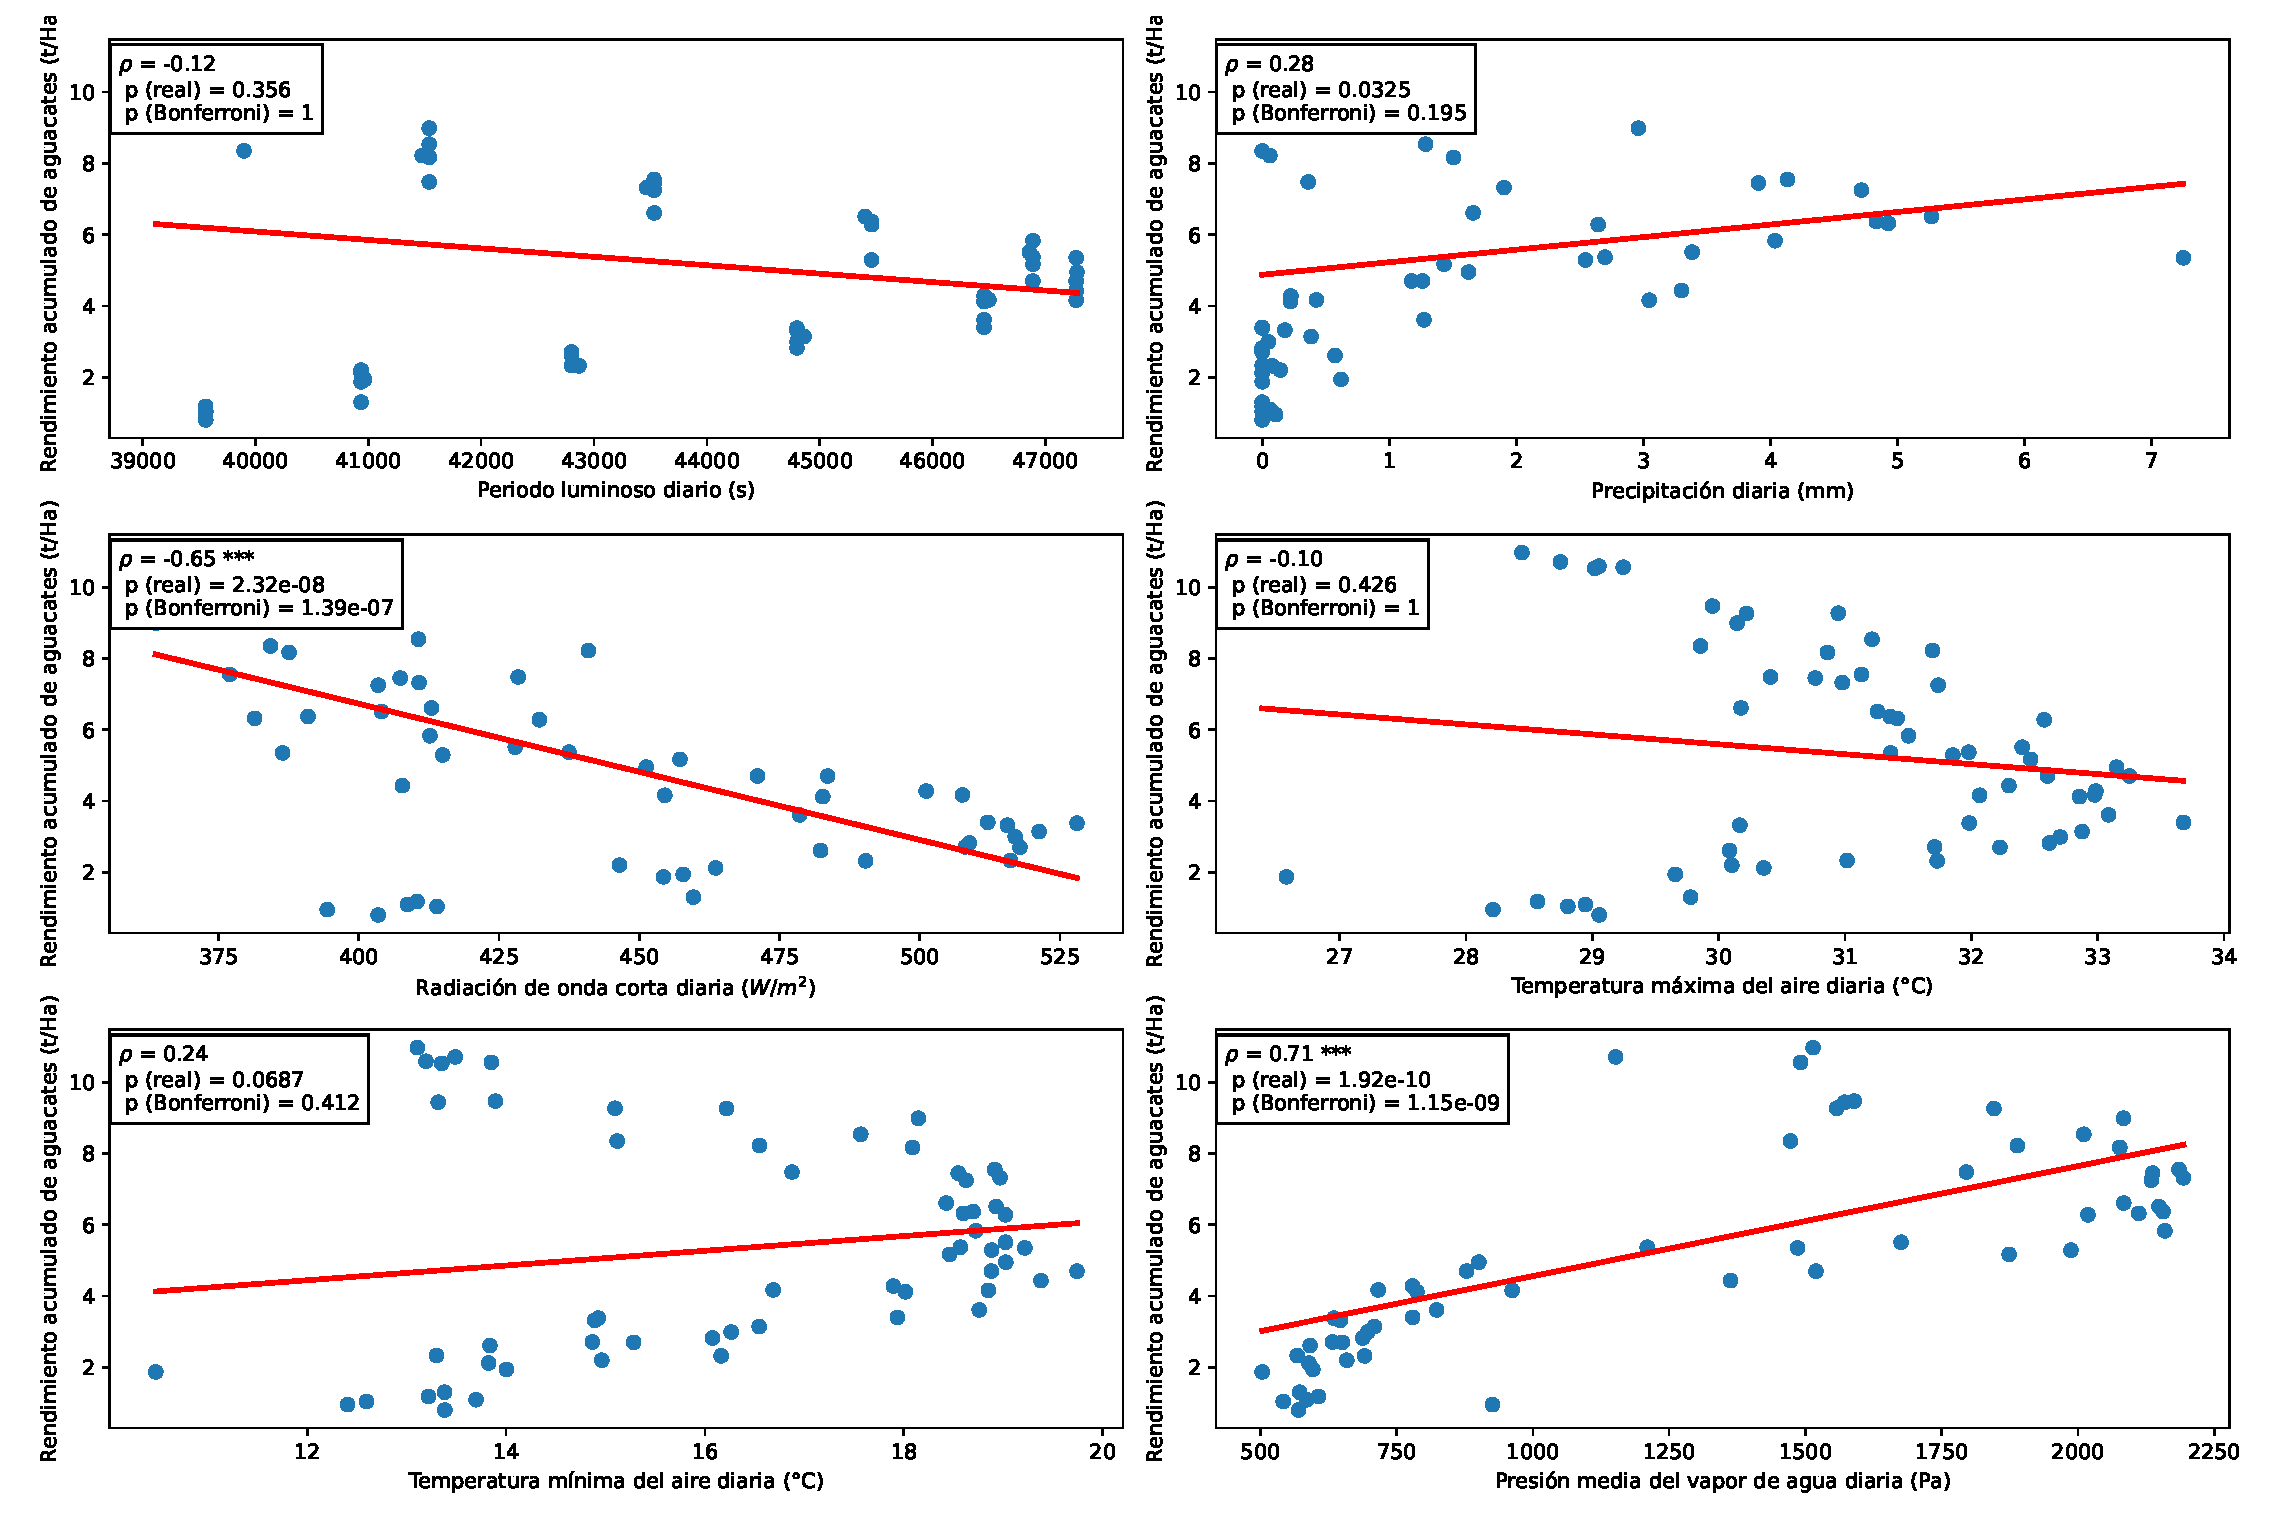
\includegraphics[width=0.8\linewidth]{Images/Effect_on_CumulativePerformance_Tacambaro.eps}
}
%no space
\hfill
\subfloat[Los Reyes]{\label{fig:CorrelacionRendimientoAcumulado_LosReyes}
\centering
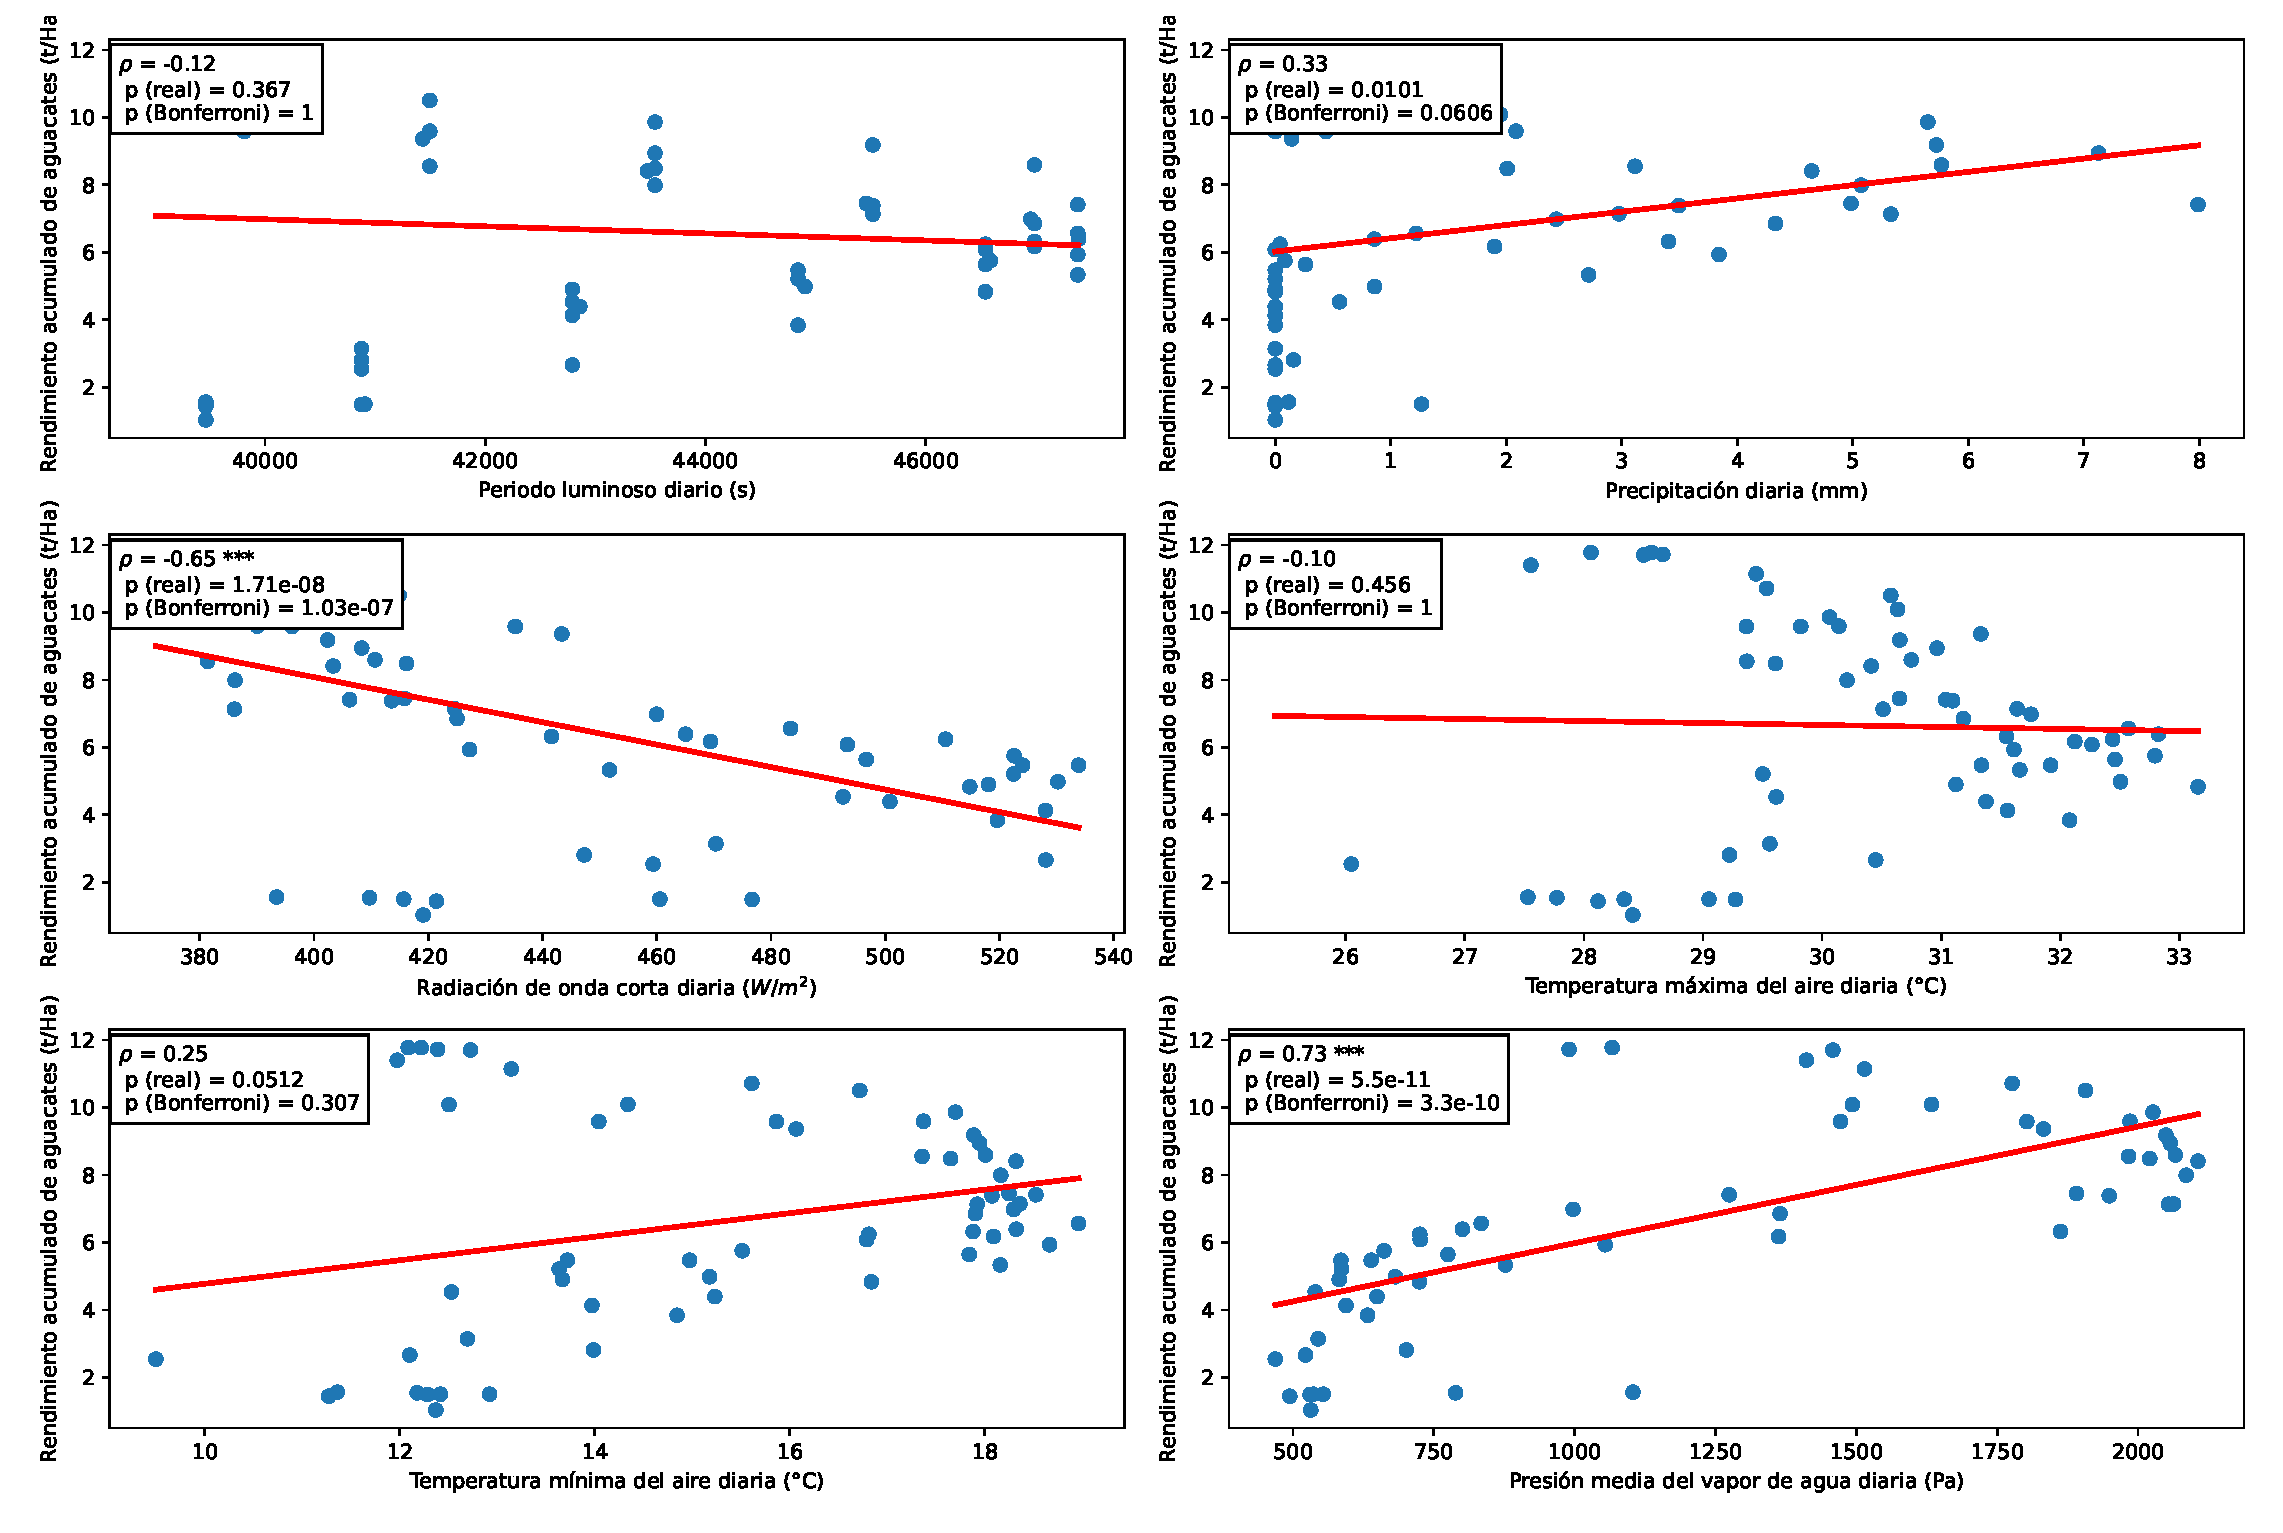
\includegraphics[width=0.8\linewidth]{Images/Effect_on_CumulativePerformance_LosReyes.eps}
}
\caption{Análisis de correlación entre las variables meteorológicas y el rendimiento acumulado de aguacates. La Figura \ref{fig:CorrelacionRendimientoAcumulado_Tacambaro} ilustra los resultados obtenidos para Tacámbaro; mientras que, la Figura \ref{fig:CorrelacionRendimientoAcumulado_LosReyes} muestra lo obtenido para Los Reyes. Se aplicaron correlaciones de Spearman con corrección de Bonferroni y su significancia estadística se denota a través de * ($p<0.05$), ** ($p<0.01$) y *** ($p<0.001$). Figura construida a partir de los datos disponibles en \cite{AvanceSiembrasCosechas} y \cite{Rodriguez-Moreno_2021}.}
\label{fig:CorrelacionRendimientoAcumulado}
\end{figure}

%Conagua datos meterológicos
Durante la exploración bibliográfica se observó un bajo número de trabajos enfocados en el pronóstico de eventos relacionados con la siembra, floración o cosecha. El trabajo de Salazar--García \textit{et al.} (2018) \cite{Salazar_2018}, por ejemplo, emplea el concepto de días de frío acumulado, una herramienta similar a la empleada por Elnesr \textit{et al.} \cite{Elnesr_2016, Elnesr_2013}, para predecir el desarrollo de las estructuras anatómicas que dan paso a las flores del aguacate a través de considerar la temperatura máxima del aire y un modelo de regresión.\\

Por otra parte, Castaño--Robayo \textit{et al.} (2022) \cite{Castaño_2022} realiza un estudio comparativo de métodos provenientes de machine learning para predecir la capacidad del suelo para retener e intercambiar nutrientes a las plantas de aguacate a través de analizar la capacidad de intercambio catiónico e identificar las variables edáficas que intervienen para implementarlas en modelos supervisados.\\ 


Además, Akin \textit{et al.} (2017) \cite{Akin_2017} estudia series de tiempo sobre producción de aguacates en Turquía, desde 1988 a 2015, y caracteriza su comportamiento como series no estacionarias, con tendencia y no estacionalidad, por lo que propone la implementación del modelo de suavizamiento exponencial de Brown como un método confiable para la predicción de la producción de aguacates.\\

Similarmente, el trabajo de Arizmendi-Peralta (2024) \cite{ARIZMENDIPERALTA2024} también se centra en el pronóstico de producción de aguacates a partir de emplear datos recolectados por sensores ensamblados y programados por cuenta propia e instalados en una huerta del municipio de Huitzilac, Morelos. Con los datos recabados, implementa tanto algoritmos supervisados como no supervisados para generar las estimaciones.\\

Asimismo, en el trabajo de Mosquera \textit{et al.} (2015) \cite{Mosquera_2015} se plantea un modelo de regresión cuadrática para analizar la producción de aguacates, a nivel de huerta y con árboles de misma edad, para detectar una baja en su rendimiento causada por la enfermedad de la marchitez del laurel, que es causada por un hongo, y proceder a retirar los árboles en cuestión.\\

Por otra parte, el proceso productivo no termina con la cosecha, sino que también incluye el almacenamiento. De esta manera, Pérez \textit{et al.} (2004) \cite{Perez_2004} propone un modelo basado en la temperatura de los almacenes para estimar el tiempo que el aguacate perdurará hasta estar disponible en el mercado.\\

El resto de trabajos que fueron explorados durante la revisión bibliográfica centran su estudio en estimar la madurez del fruto, su calidad, detectar plagas e infecciones, densidad de flores y ventas. La mayoría de estos trabajos emplean análisis de imágenes satelitales, infrarrojas y radiografías, por lo que el costo computacional a gran escala puede resultar elevado. \\


De esta manera, este trabajo tiene como objetivo el desarrollo e implementación de herramientas, metodologías y algoritmos de aprendizaje automático con la finalidad de pronosticar la producción, temporadas de siembra, floración y cosecha en función del análisis de datos agroclimáticos históricos.  De manera tal que sea posible tomar decisiones respecto al cuidado de cultivos; por ejemplo, al combinar los tipos de riego, proteger del calor y quemaduras por el sol a los tallos y ramas  o cubrir las bases de los árboles para preservar la humedad, maximizando la supervivencia y producción, implicando un mayor flujo económico.\\

En conclusión, este trabajo pretende contribuir al fortalecimiento y desarrollo de la industria agrícola nacional e internacional mediante la aplicación de la ciencia de datos. La agricultura garantiza el abasto de alimentos y materia prima para diversos sectores productivos, y la implementación de métodos actuales es capaz de minimizar los efectos del cambio climático, implicando mejoras en la seguridad alimentaria y la economía.

